\chapter{Part II(d) - Processor, I/Os, and Exceptions W - 5.1}

\section{Exceptions, Interrupts, Faults, Traps, and Checks}

\paragraph{Control Flow}
Under normal circumstances, the \textit{control flow}—the sequence of instructions executed by a program—is fully determined by the programmer. This includes the use of jumps, branches, and procedure calls.

\paragraph{Exceptions}
Exceptions represent a deviation from the normal control flow. They are triggered by \textbf{special conditions} that are not explicitly defined in the program. When an exception occurs, the control flow changes unexpectedly, and the program must respond accordingly.

\paragraph{Exception Handlers}
To manage exceptions, \textit{exception handlers} are invoked. These are specialized functions designed to take appropriate actions when an exception arises. An example of this is \textbf{I/O interrupts}, which signal specific events related to input/output operations.

\paragraph{Naming Conventions}
The terminology for exceptions and related events varies widely across systems. For clarity, we adopt the following convention based on RISC-V and the COD:
\begin{itemize}
    \item \textbf{Exceptions:} A general term encompassing all control flow deviations.
    \item \textbf{Interrupts:} A specific type of exception generated outside the processor.
\end{itemize}
Thus far, interrupts are the only form of exception encountered.
\newpage
\subsection{Undefined Instruction}

Undefined instructions are instructions that the controller does not recognize, as they do not correspond to any valid operation in the Instruction Register (IR). These scenarios require special handling to ensure system stability and proper exception processing.

\vspace{0.5cm}
\begin{minipage}[htp]{0.35\textwidth}
- \textbf{Detection:} When an undefined instruction is detected in the IR, the controller generates a signal (\texttt{undef}) indicating the presence of an invalid operation. \\ 
- \textbf{Exception Handling:} The Program Counter (PC) is updated to the address of the Exception Handler to manage the undefined instruction. This involves: \\
\begin{itemize}
\item Saving the current PC for potential recovery.
\item Redirecting the control flow to the exception handler's address using multiplexer logic.
\end{itemize}
- \textbf{Control Logic:} The system leverages the Next PC Logic to determine whether the next instruction comes from the regular PC logic or the exception handler, based on the \texttt{undef} signal or an external interrupt (IRQ).
\end{minipage}
\hfill
\vline
\hfill
\begin{minipage}[htp]{0.55\textwidth}
    \begin{center}
        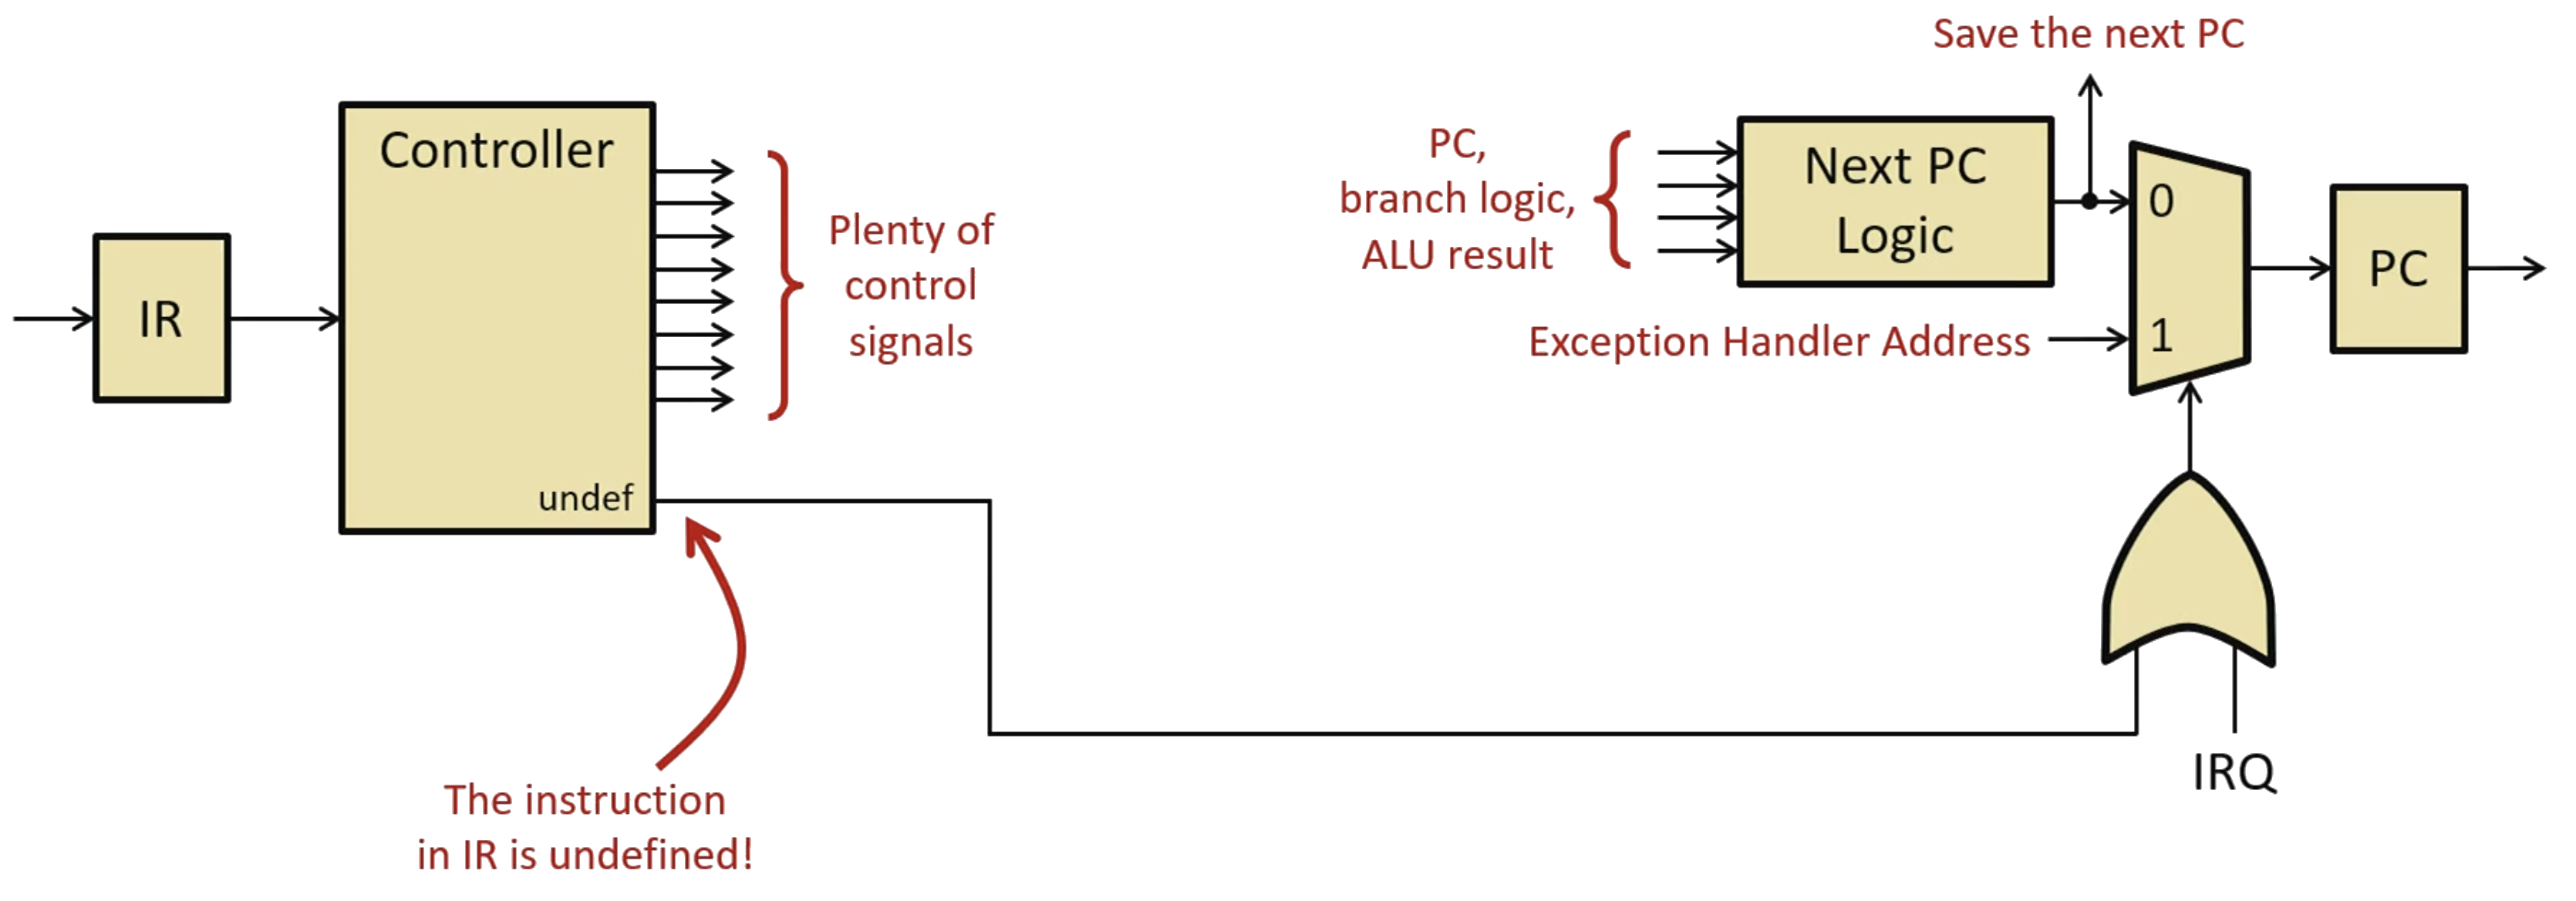
\includegraphics[width=1.1\textwidth]{chapters/chapter2d/images/undefined.png}
    \end{center}
\end{minipage} \\
\vspace{0.5cm}
- \textbf{Synchronous Nature:} These exceptions occur at a specific point in the program, precisely where the undefined instruction resides. This predictable behavior ensures that if the program is re-executed from the same initial state, the exception will occur at the exact same point, making debugging more straightforward. \\ \vspace{0.5cm}
- \textbf{Immediate Handling:} Serving the exception before executing the next instruction allows advanced features, such as efficient error recovery and the potential to extend system capabilities.
\vspace{0.5cm}
This mechanism ensures that undefined instructions do not disrupt the execution flow and are handled systematically, enabling robust error recovery and system stability.

\subsection{Optional \texttt{fadd.s} Instruction}

Suppose we want to include a floating-point addition instruction, denoted as:
\begin{assembly}
fadd.s rd, rs1, rs2
\end{assembly}

- Some processors might include a specialized ALU to support this instruction, whereas \textbf{cheaper processors do not}. \\ \vspace{7px}
- For processors that lack support for this instruction, its execution would trigger an \textit{undefined instruction exception}, which invokes a handler. \\ \vspace{7px}
- The handler can \textbf{emulate} the behavior of the \texttt{fadd.s} instruction, ensuring compatibility across processors. \\ \vspace{7px}

\subsection{Outline of an Undefined Instruction Handler}
To handle an undefined instruction, such as \texttt{fadd.s}, the following steps wouls be executed:
\begin{itemize}
    \item[] \textbf{Save all registers} on the stack that the handler or its callees might modify.
    \begin{itemize}
        \item Note: Standard calling conventions do not apply.
    \end{itemize}
    \item[] \textbf{Retrieve the problematic instruction}:
    \begin{itemize}
        \item If the program counter (PC) is saved, load the instruction from the corresponding address.
    \end{itemize}
    \item[] \textbf{Decode the instruction} in software and identify it as \texttt{fadd.s}.
    \item[] \textbf{Read the source registers} (operands) and either:
    \begin{itemize}
        \item Call a library function, or
        \item Implement the floating-point addition in software.
    \end{itemize}
    \item[] \textbf{Store the result} in the destination register.
    \item[] \textbf{Update the program counter (PC)} to point to the next instruction.
    \item[] \textbf{Jump to the updated PC} to resume execution.
\end{itemize}

\section{Exceptions and Interrupts}
Exceptions, interrupts, and related mechanisms handle critical events during execution. Key use cases include:
\begin{itemize}
    \item[] \textbf{I/O Requests:} Processing data or new inputs.
    \item[] \textbf{Timer Interrupts:} Handling time-based events.
    \item[] \textbf{Undefined Instructions:} E.g., unsupported floating-point operations.
    \item[] \textbf{Arithmetic Faults:} Errors like division by zero.
    \item[] \textbf{Memory Violations:} Unauthorized access to restricted memory.
    \item[] \textbf{Debugging:} Breakpoints and execution control.
    \item[] \textbf{Hardware Failures:} Malfunctions such as power loss.
\end{itemize}
\subsection{A Possible Classification of Exceptions}
\begin{center}
    \begin{tabular}{|l|l|l|l|}
    \hline
    \textbf{Type}                     & \textbf{Synchronous?} & \textbf{Coerced?}      & \textbf{Resume?} \\ \hline
    I/O request                       & Asynchronous          & Coerced               & Resume           \\ \hline
    Invoke OS                         & Synchronous           & User requested        & Resume           \\ \hline
    Trace instruction                 & Synchronous           & User requested        & Resume           \\ \hline
    Breakpoint                        & Synchronous           & User requested        & Resume           \\ \hline
    Page fault                        & Synchronous           & Coerced               & Resume           \\ \hline
    Misaligned access                 & Synchronous           & Coerced               & Resume           \\ \hline
    Memory protection violation       & Synchronous           & Coerced               & Terminate        \\ \hline
    Bus error                         & Synchronous           & Coerced               & Terminate        \\ \hline
    Arithmetic fault                  & Synchronous           & Coerced               & Terminate        \\ \hline
    Undefined instruction             & Synchronous           & Coerced               & Terminate        \\ \hline
    Hardware malfunction              & Asynchronous          & Coerced               & Terminate        \\ \hline
    Power failure                     & Asynchronous          & Coerced               & Terminate        \\ \hline
    \end{tabular}
\end{center}

\begin{itemize}
    \item \textbf{Synchronous?} Indicates whether the exception occurs as a direct result of the execution flow (synchronous) or independently of it (asynchronous).
    \item \textbf{Coerced?} Specifies whether the exception is forced by the system (coerced) or triggered by a user request.
    \item \textbf{Resume?} Denotes whether the system can continue executing after handling the exception (resume) or must terminate.
\end{itemize}

\subsection{Watchpoint}
A \textbf{watchpoint} is a debugging feature in a processor architecture that monitors specific registers and triggers an exception when predefined conditions are met. This mechanism allows developers to track changes in critical registers and execute exception handlers when necessary. \\
\begin{minipage}[htp]{0.45\textwidth}
\small
\textbf{Key Components}
\begin{itemize}
    \item[-] \textbf{Register File:} Contains the set of registers, including special registers that can be configured by the user.
    \item[-] \textbf{Watchpoint Logic:} Compares the monitored \textit{register} and its \textit{value} with user-defined conditions.
    \item[-] \textbf{Next PC Logic:} Determines the next program counter (PC) value based on standard flow or exception handling.
\end{itemize}
\textbf{Functionality}
\begin{itemize}
    \item[-] When an instruction writes a specific \textit{value} into the monitored \textit{register}, the watchpoint logic evaluates the predefined conditions.
    \item[-] If the conditions are met, the system triggers an exception by redirecting the program counter to the \textit{exception handler address}.
    \item[-] Otherwise, normal program execution continues.
\end{itemize}
\end{minipage}
\hfill
\vline
\hfill
\begin{minipage}[htp]{0.45\textwidth}
\begin{center}
    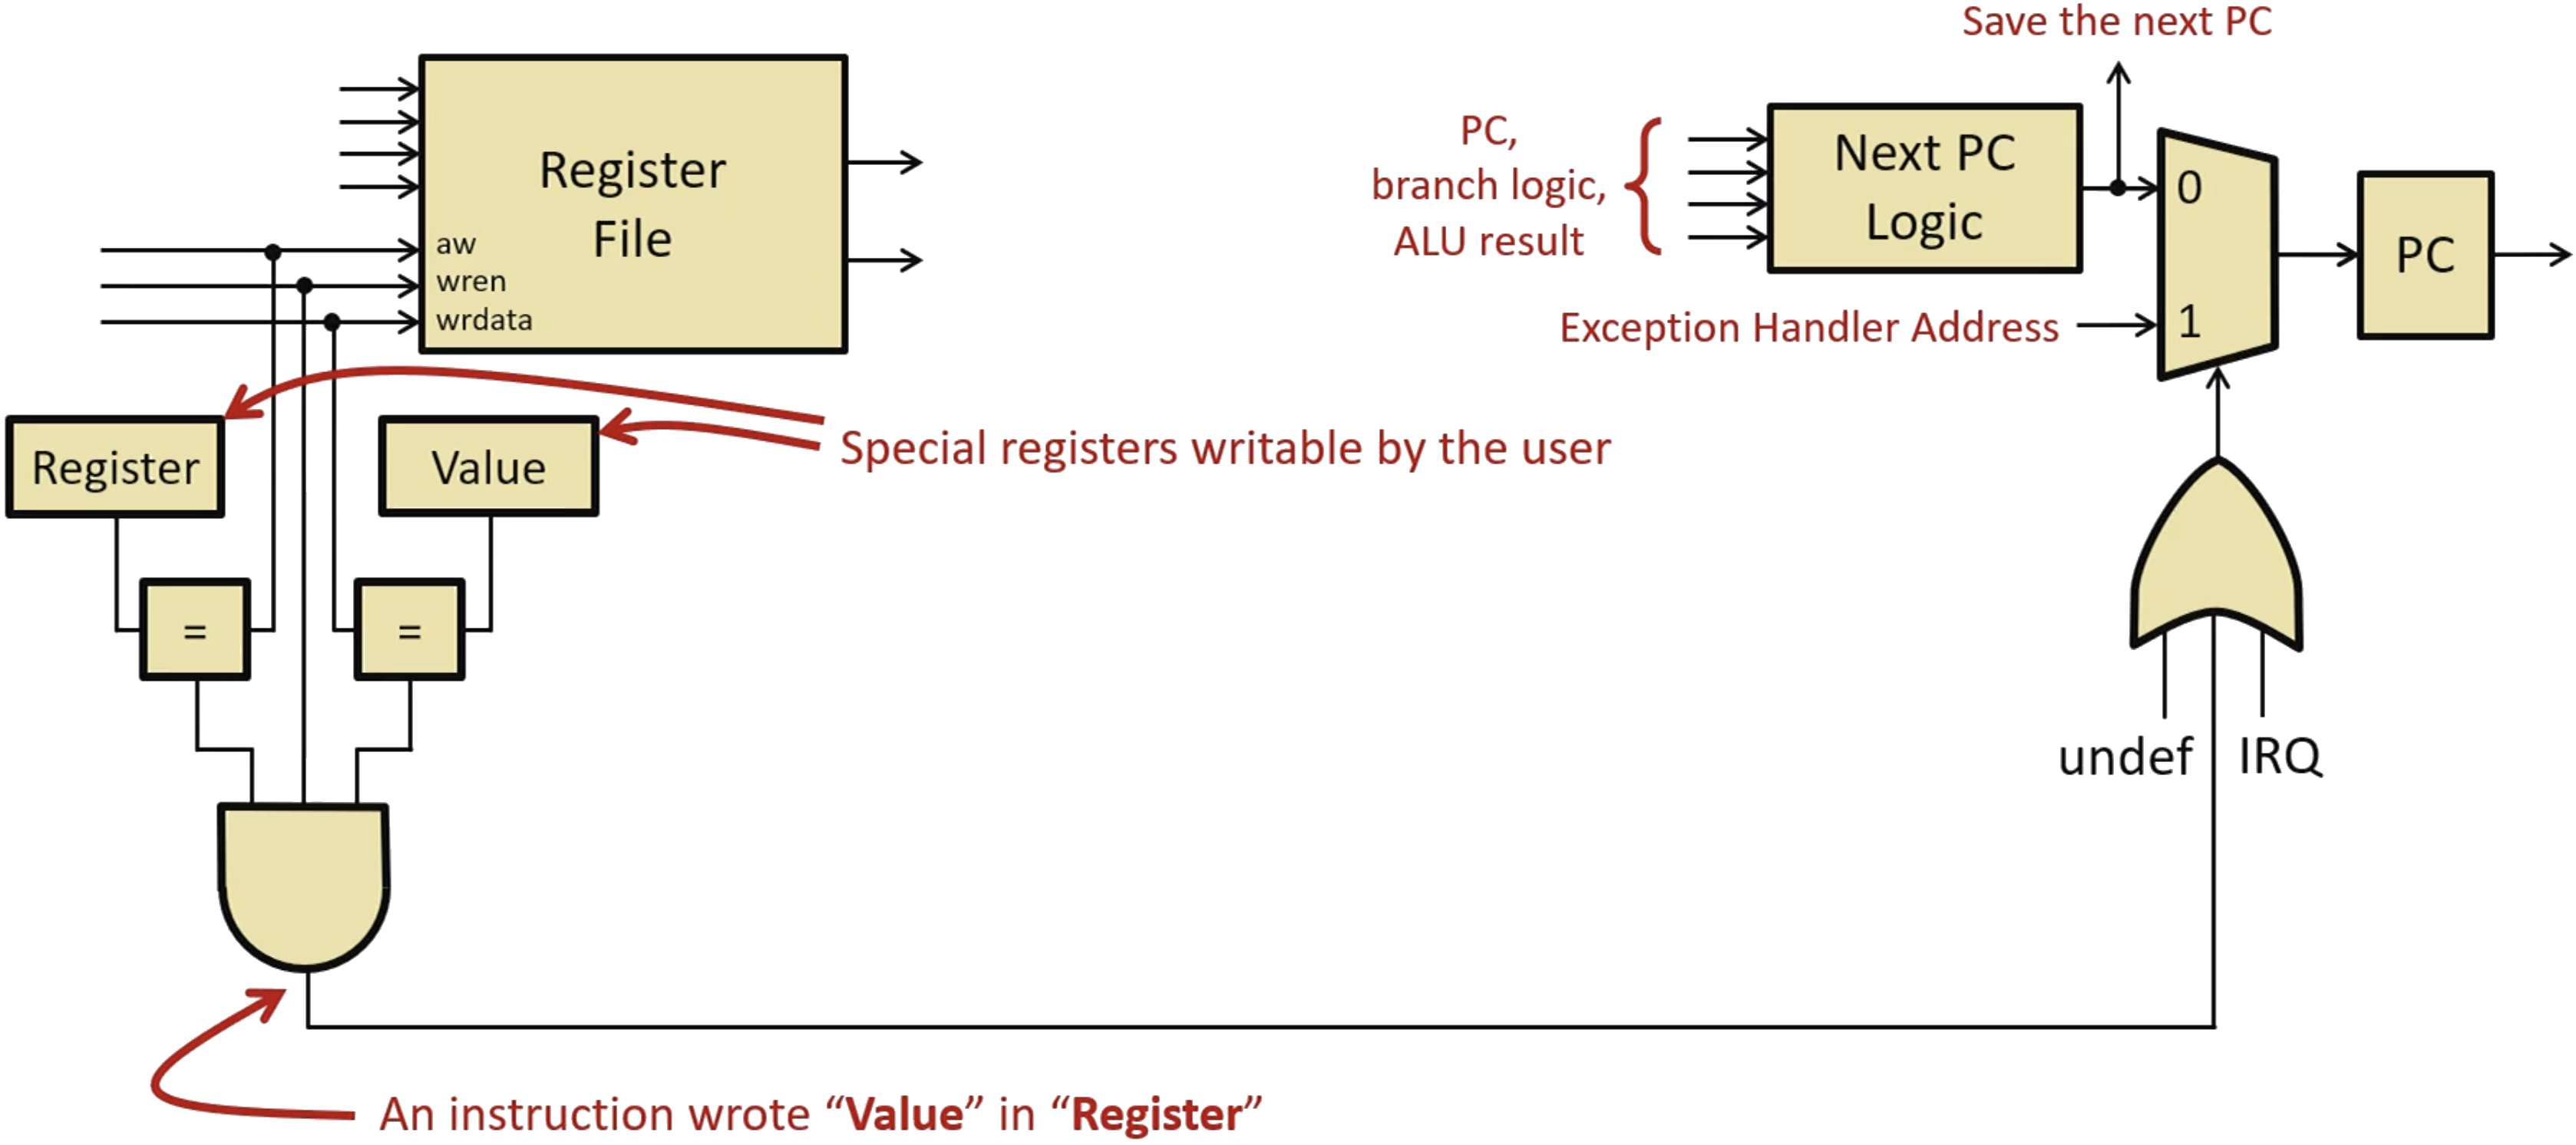
\includegraphics[width=1.1\textwidth]{chapters/chapter2d/images/watchpoint.png}
\end{center}
\end{minipage}

\subsection{Raising Exceptions}
To handle exceptions, the processor must be able to provide which exact exception occurred. 
\begin{itemize}
    \item[] \textbf{Saving the Address:} The address of the current or next instruction must be stored in a dedicated register, typically the \textit{Exception Program Counter (EPC)}. This prevents overwriting the \texttt{ra} register, which is used for ordinary returns. A special instruction is required to resume execution using the \texttt{EPC}.
    \item[] \textbf{Multiple Causes:} Since exceptions can arise from various causes, a mechanism is needed to identify the source:
    \begin{itemize}
        \item A single handler address with a \textit{cause register}.
        \item A vector of handlers, where each handler corresponds to a specific cause.
    \end{itemize}
    \item[] \textbf{Nested Interrupts/Exceptions:} While handling an exception, another may occur. To manage this:
    \begin{itemize}
        \item Disable exceptions that can be suppressed (e.g., interrupts).
        \item Avoid unpreventable exceptions (e.g., division by zero or undefined instructions).
    \end{itemize}
\end{itemize}

\subsection{Assessing the Position of an Exception}
When an exception occurs, it is essential to determine the position in the instruction flow to decide the appropriate handling strategy. Some key considerations are: \\
- \textbf{Asynchronous Exceptions:} 
\begin{itemize}
    \item Identify the \textit{next instruction} to execute.
\end{itemize}
- \textbf{Synchronous Exceptions:} \\
\begin{itemize}
    \item Determine the \textit{instruction that caused the fault}.
    \begin{itemize}
        \item Restart from the faulting instruction if correction and retry are needed (e.g., invoking the operating system).
        \item Restart from the next instruction if the functionality is implemented differently (e.g., emulating an undefined instruction in software).
    \end{itemize}
\end{itemize}
- \textbf{Solutions:} \\
\begin{itemize}
    \item Reserve a dedicated ordinary register for the \textit{Exception Program Counter (EPC)} (e.g., Nios II).
    \item Store the EPC on the stack (e.g., x86).
    \item Use special registers dedicated to exception handling with specific instructions to access them (e.g., MIPS, RISC-V).
\end{itemize}
\subsection{Assessing the Cause of Exception}
To handle exceptions, the processor must pass control to the appropriate handler. The mechanism for determining and invoking the correct handler can be categorized as follows:
\begin{itemize}
    \item[] \textbf{Single Handler with Cause Register (e.g., RISC-V, MIPS):}
    \begin{itemize}
        \item The processor executes a jump to a fixed address.
        \item The handler performs the dispatching in software by reading a special \textit{cause register}.
    \end{itemize}
    \item[] \textbf{Vector of Handler Addresses (e.g., RISC-V, 68k):}
    \begin{itemize}
        \item The processor executes a jump to \texttt{mem[Exception Vector Address + (4 $\times$ Exception Number)]}.
    \end{itemize}
    \item[] \textbf{Vector of Handlers (e.g., PA-RISC 2.0, SPARC):}
    \begin{itemize}
        \item The processor directly jumps to \texttt{Exception Vector Address + (32 $\times$ Exception Number)}.
    \end{itemize}
\end{itemize}
\begin{center}
    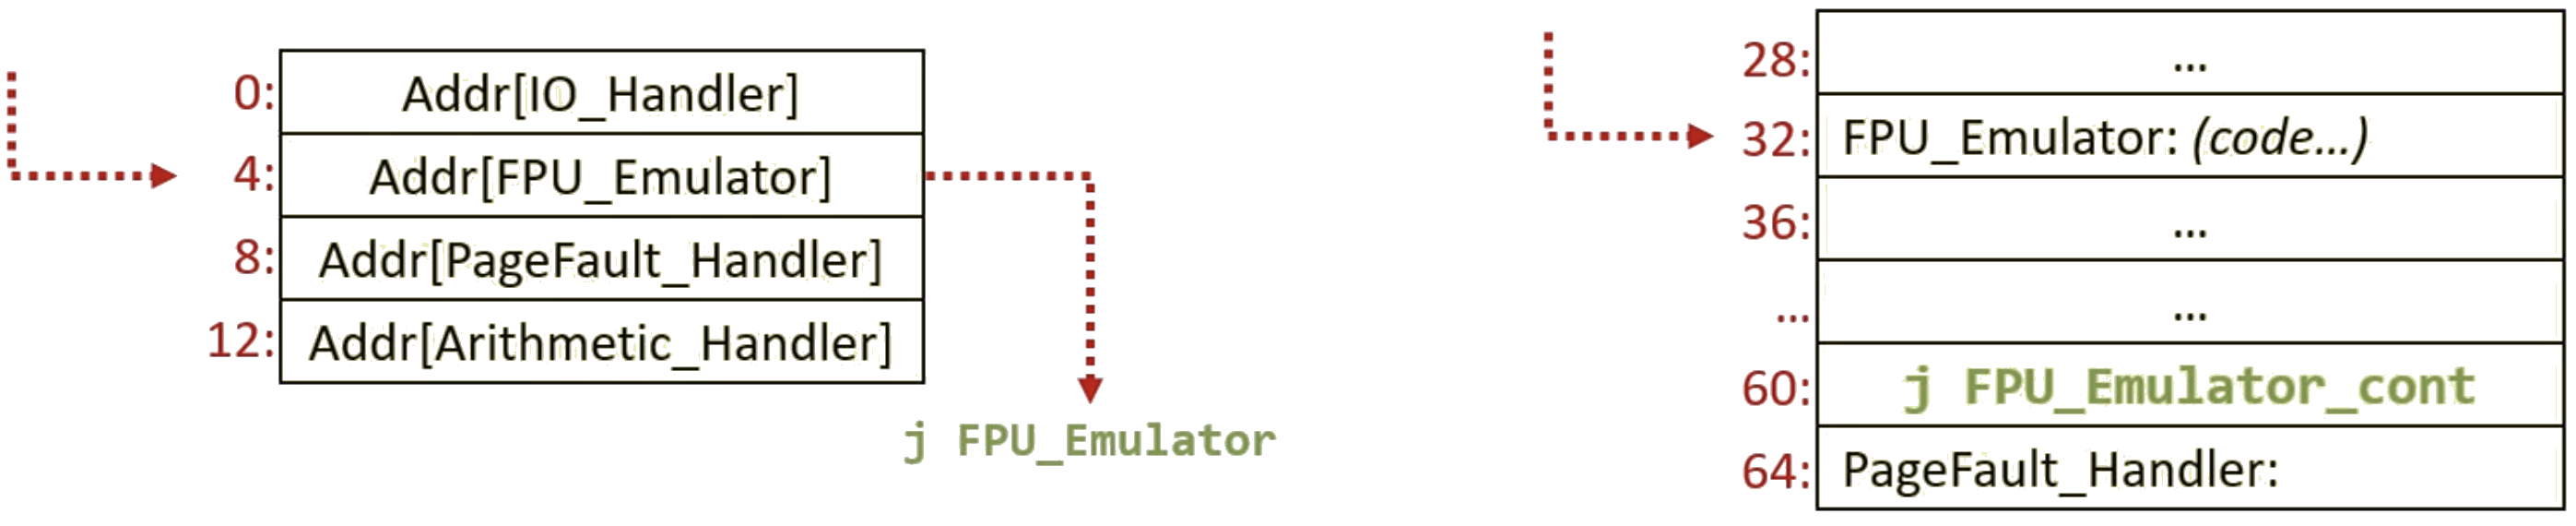
\includegraphics[width=0.65\textwidth]{chapters/chapter2d/images/position.png}
\end{center}
\subsection{RISC-V Machine-Mode Exception Handling}
\subsubsection{Control and Status Registers (CSRs)}
Control and Status Registers (CSRs) are essential for handling exceptions and managing processor states. Key registers include:

\begin{itemize}
    \item \textbf{mstatus:} Contains global interrupt enable flags (e.g., \texttt{MIE}) and status bits.
    \item \textbf{mie:} Manages individual interrupt enable bits (e.g., \texttt{MEIE}, \texttt{MTIE}).
    \item \textbf{mip:} Indicates pending interrupts (e.g., \texttt{MEIP}, \texttt{MTIP}).
    \item \textbf{mtvec:} Stores the base address for exception vectors.
    \item \textbf{mepc:} Holds the Program Counter (PC) value at the time of an exception.
    \item \textbf{mcause:} Stores the cause of the exception, differentiating between interrupts and exception codes.
\end{itemize}

\subsubsection{Instructions for Accessing CSRs}
The following instructions facilitate read/write operations on CSRs:

\begin{center}
\begin{tabular}{|l|l|l|}
\hline
\textbf{Instruction} & \textbf{Pseudocode} & \textbf{Meaning} \\
\hline
\texttt{csrrw rd, csr, rs1} & \texttt{rd $\leftarrow$ csr; csr $\leftarrow$ rs1} & Read/Write CSR \\
\texttt{csrrs rd, csr, rs1} & \texttt{rd $\leftarrow$ csr; csr $\leftarrow$ csr | rs1} & Read/Set Bits CSR \\
\texttt{csrrc rd, csr, rs1} & \texttt{rd $\leftarrow$ csr; csr $\leftarrow$ csr \& (~rs1)} & Read/Clear Bits CSR \\
\texttt{csrrwi rd, csr, imm} & \texttt{rd $\leftarrow$ csr; csr $\leftarrow$ imm} & Read/Write CSR (Immediate) \\
\texttt{csrrsi rd, csr, imm} & \texttt{rd $\leftarrow$ csr; csr $\leftarrow$ csr | imm} & Read/Set Bits CSR (Immediate) \\
\texttt{csrrci rd, csr, imm} & \texttt{rd $\leftarrow$ csr; csr $\leftarrow$ csr \& (~imm)} & Read/Clear Bits CSR (Immediate) \\
\hline
\end{tabular}
\end{center}

\subsubsection{Returning from Exceptions}
The \texttt{mret} instruction is used to return from machine mode:
\begin{itemize}
    \item Restores the previous interrupt enable state (\texttt{mstatus.MIE $\leftarrow$ mstatus.MPIE}).
    \item Updates the Program Counter (\texttt{pc $\leftarrow$ mepc}).
\end{itemize}

\subsection{RISC-V Interrupt and Exception Codes}

The RISC-V architecture defines a set of interrupt and exception codes, categorized based on their source and purpose. These codes are represented in the \texttt{mcause} register, with the highest bit (\texttt{mcause[31]}) distinguishing between interrupts and exceptions.

\subsubsection*{Interrupts}
Interrupts occur asynchronously and are triggered by external or internal events. Key examples include:
\begin{itemize}
    \item \textbf{Supervisor software interrupt (Code 1):} Triggered by software at the supervisor level.
    \item \textbf{Machine software interrupt (Code 3):} Triggered by software at the machine level.
    \item \textbf{Supervisor timer interrupt (Code 5):} Indicates a timer interrupt at the supervisor level.
    \item \textbf{Machine timer interrupt (Code 7):} Indicates a timer interrupt at the machine level.
    \item \textbf{Supervisor external interrupt (Code 9):} Indicates an external I/O interrupt at the supervisor level.
    \item \textbf{Machine external interrupt (Code 11):} Indicates an external I/O interrupt at the machine level.
\end{itemize}

\subsubsection*{Exceptions}
Exceptions are synchronous events that occur during instruction execution. Common examples include:
\begin{itemize}
    \item \textbf{Instruction address misaligned (Code 0):} Caused by an attempt to fetch an instruction from a misaligned address.
    \item \textbf{Instruction access fault (Code 1):} Occurs when an instruction fetch violates access permissions.
    \item \textbf{Illegal instruction (Code 2):} Raised when an undefined or restricted instruction is executed.
    \item \textbf{Breakpoint (Code 3):} Triggered by a breakpoint instruction for debugging.
    \item \textbf{Page faults:}
    \begin{itemize}
        \item \textbf{Instruction page fault (Code 12):} Indicates a fault during instruction fetch due to virtual memory issues.
        \item \textbf{Load page fault (Code 13):} Raised during a load operation when a page-related fault occurs.
        \item \textbf{Store page fault (Code 15):} Raised during a store operation when a page-related fault occurs.
    \end{itemize}
\end{itemize}

Understanding and properly handling these interrupts and exceptions is crucial for effective RISC-V programming and system design.

\subsection{Possible Undefined Instruction Handler}
Below is a possible implementation of an undefined instruction handler in RISC-V assembly:
\begin{center}
    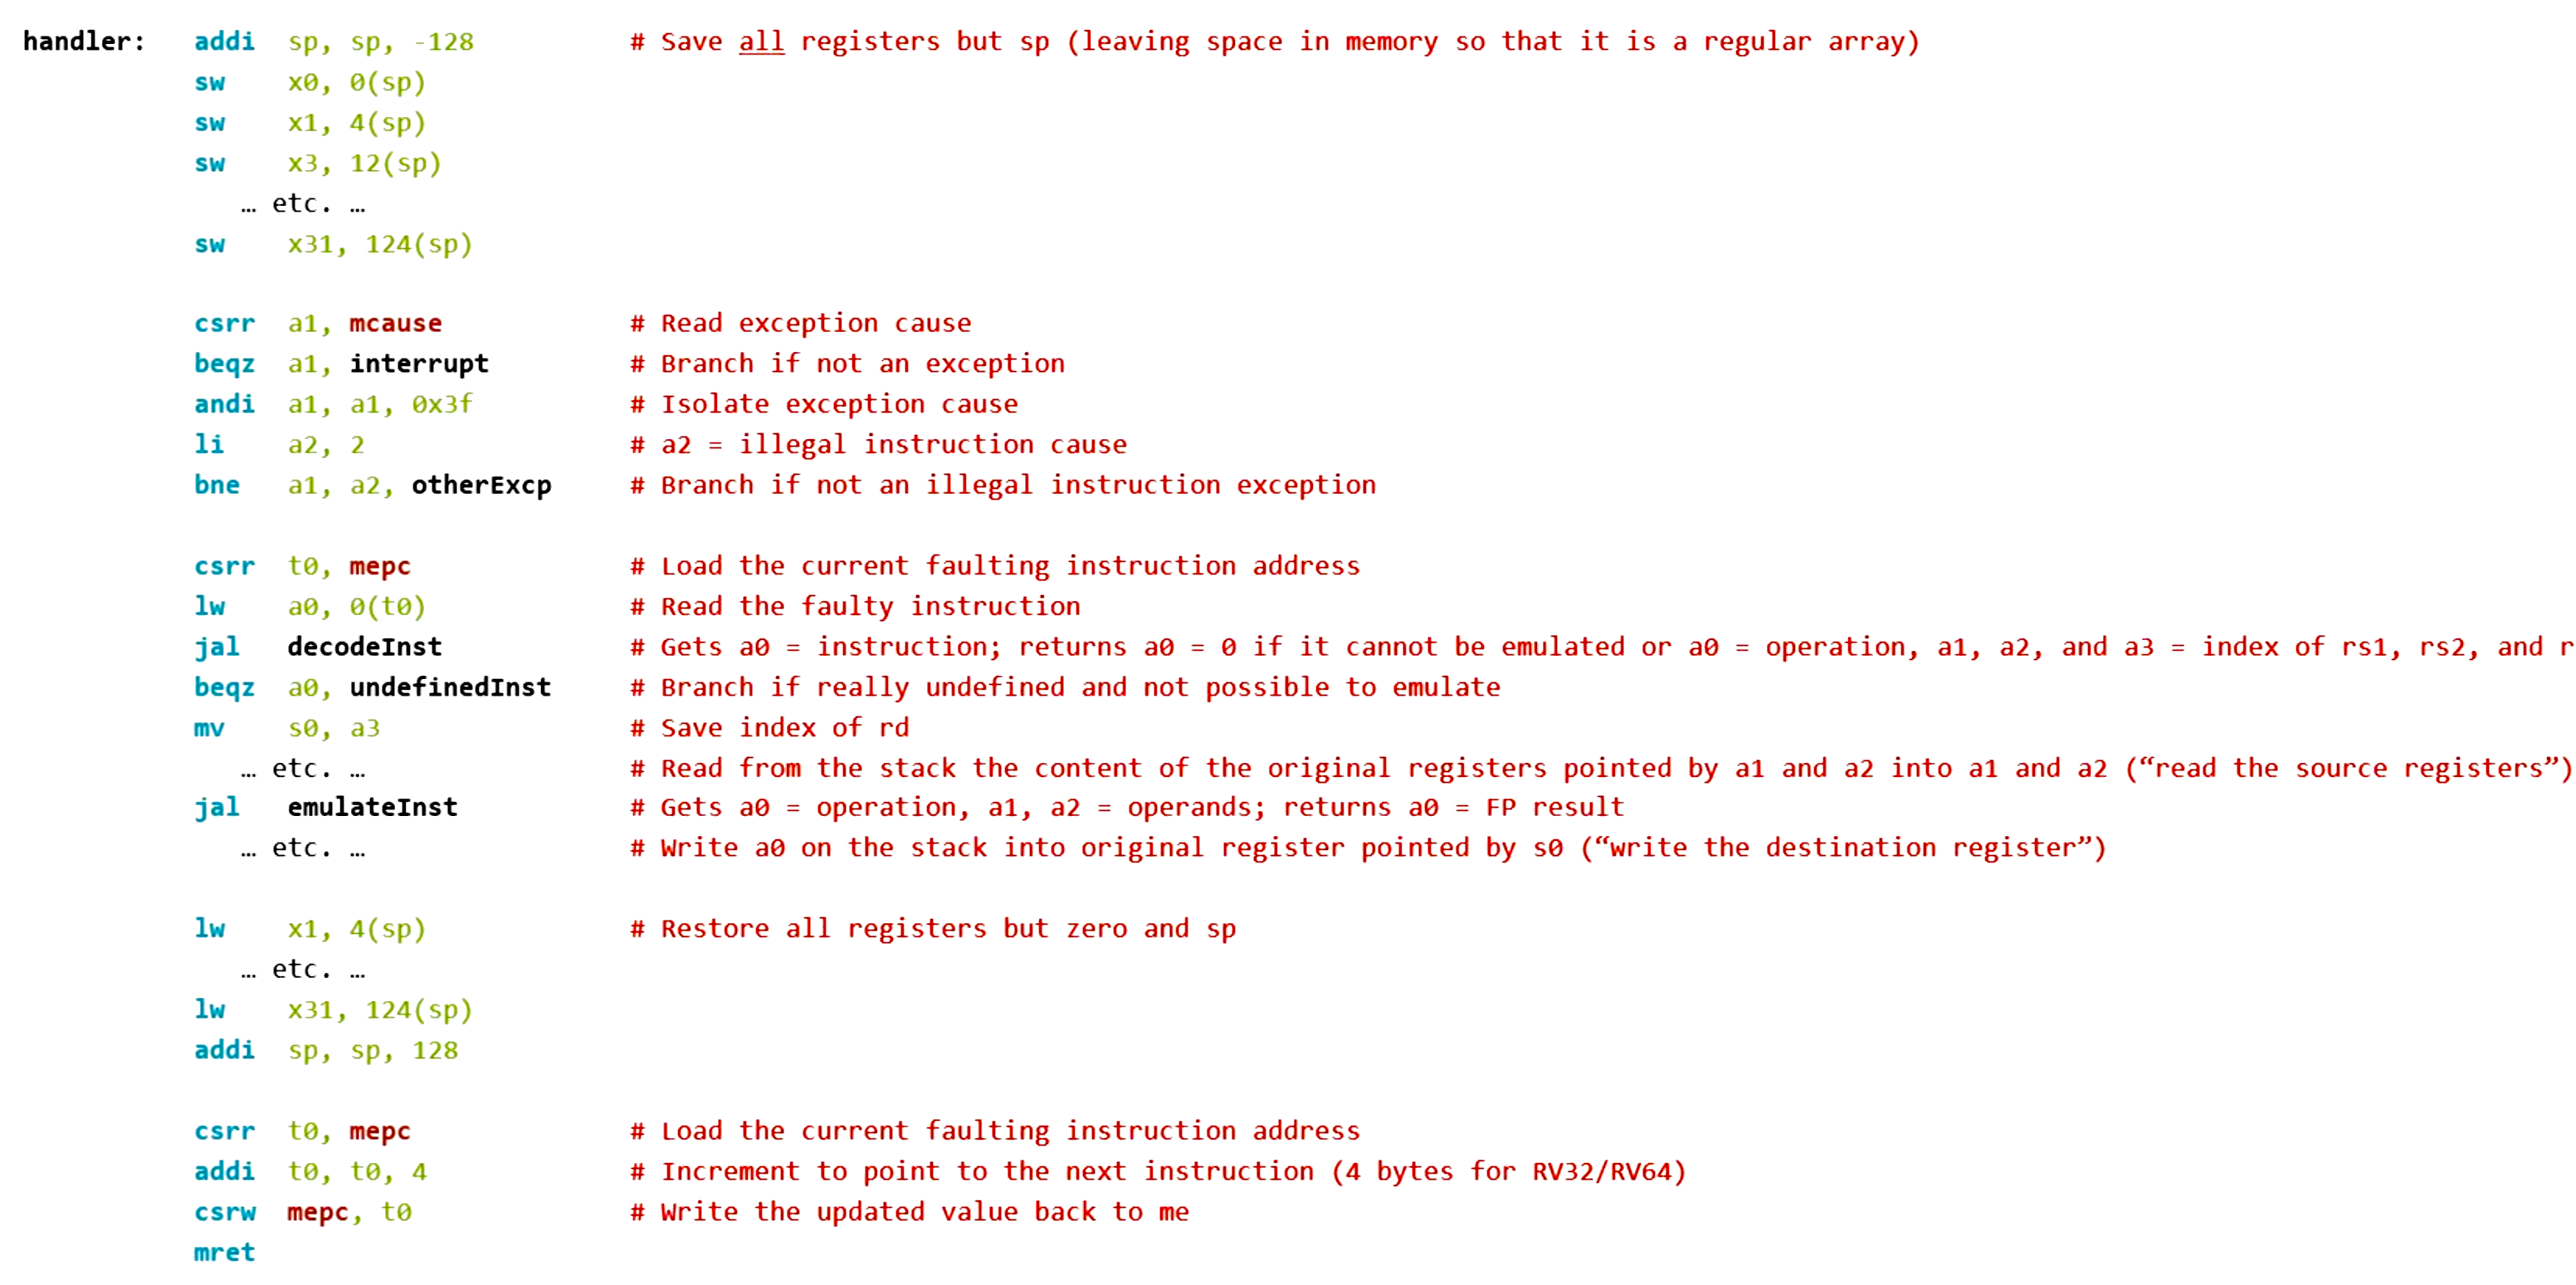
\includegraphics[width=1\textwidth]{chapters/chapter2d/images/instr_handler.png}
\end{center}

\subsection{RISC-V Machine-Mode Interrupt Handling}

In RISC-V architecture, machine-mode interrupt handling is managed through three key control and status registers: \texttt{mie}, \texttt{mip}, and \texttt{mstatus}. These registers play distinct roles in enabling, monitoring, and controlling interrupts.

\begin{itemize}
    \item \textbf{\texttt{mie} (Machine Interrupt Enable):} 
    This register determines which interrupts the processor can take and which it must ignore. Key bits include:
    \begin{itemize}
        \item \texttt{MEIE}: Enables machine-level external interrupts.
        \item \texttt{MTIE}: Enables machine-level timer interrupts.
    \end{itemize}

    \item \textbf{\texttt{mip} (Machine Interrupt Pending):} 
    This register lists the interrupts that are currently pending. Key bits include:
    \begin{itemize}
        \item \texttt{MEIP}: Indicates a pending machine-level external interrupt.
        \item \texttt{MTIP}: Indicates a pending machine-level timer interrupt.
    \end{itemize}

    \item \textbf{\texttt{mstatus} (Machine Status):} 
    This register contains the global interrupt enable flag and other state information. Important fields include:
    \begin{itemize}
        \item \texttt{MIE}: Globally enables interrupts when set to 1, and disables them when set to 0.
        \item \texttt{MPIE}: Holds the value of \texttt{MIE} prior to a trap.
    \end{itemize}
\end{itemize}

The diagram below illustrates the structure of these registers:
\begin{center}
    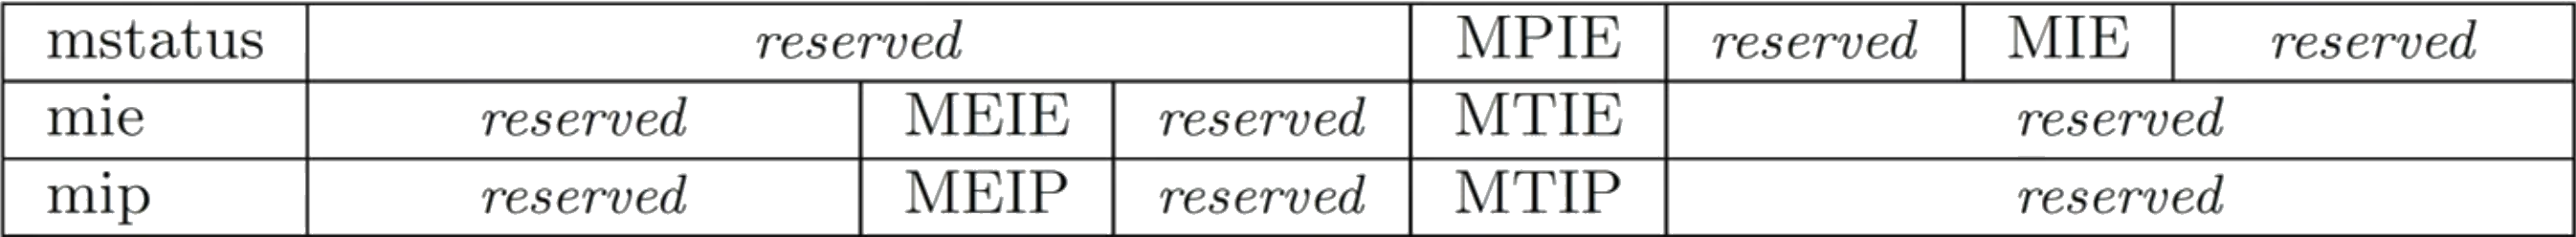
\includegraphics[width=0.85\textwidth]{chapters/chapter2d/images/int_handl_reg.png}
\end{center}

These registers provide the foundation for interrupt handling in machine mode, ensuring efficient and precise interrupt management.

\section{The Stack Problem}
A few weeks ago, we discussed a potential issue with the stack, what was, "What should we do when the stack hits its limit?" \\
We might be able to find a solution to this problem now.
\begin{center}
    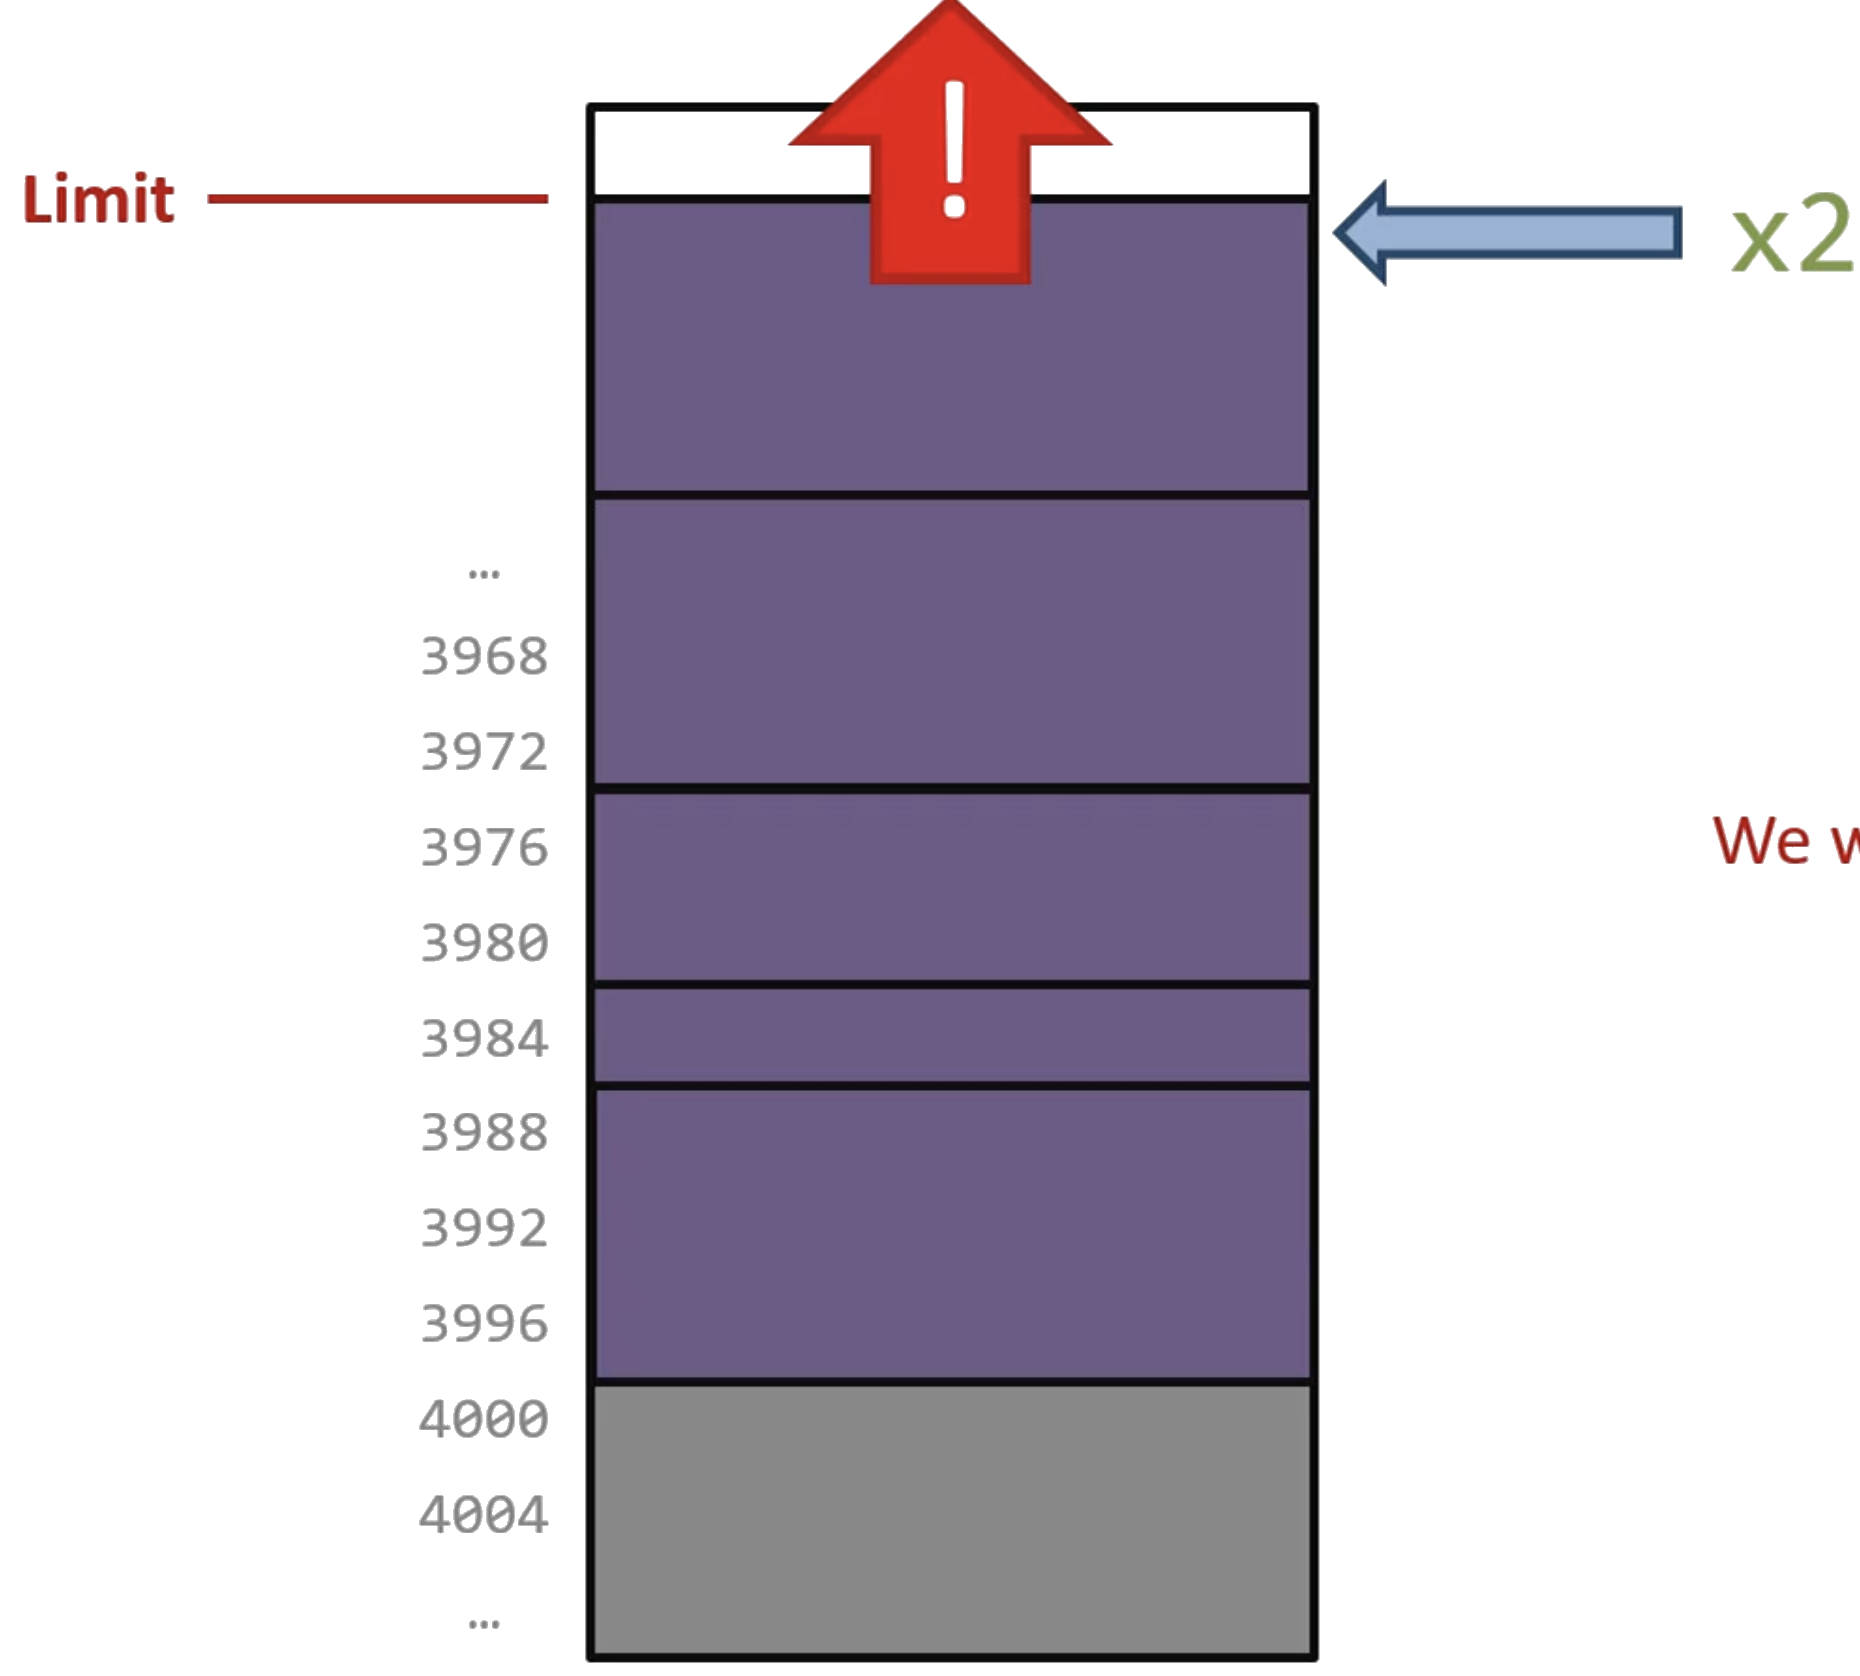
\includegraphics[width=0.35\textwidth]{chapters/chapter2d/images/limit_stack.png}
\end{center}

\newpage
\subsection{Stack-Full Detection ?}
To detect when the stack is full, we can use a watchpoint. \\
\begin{center}
    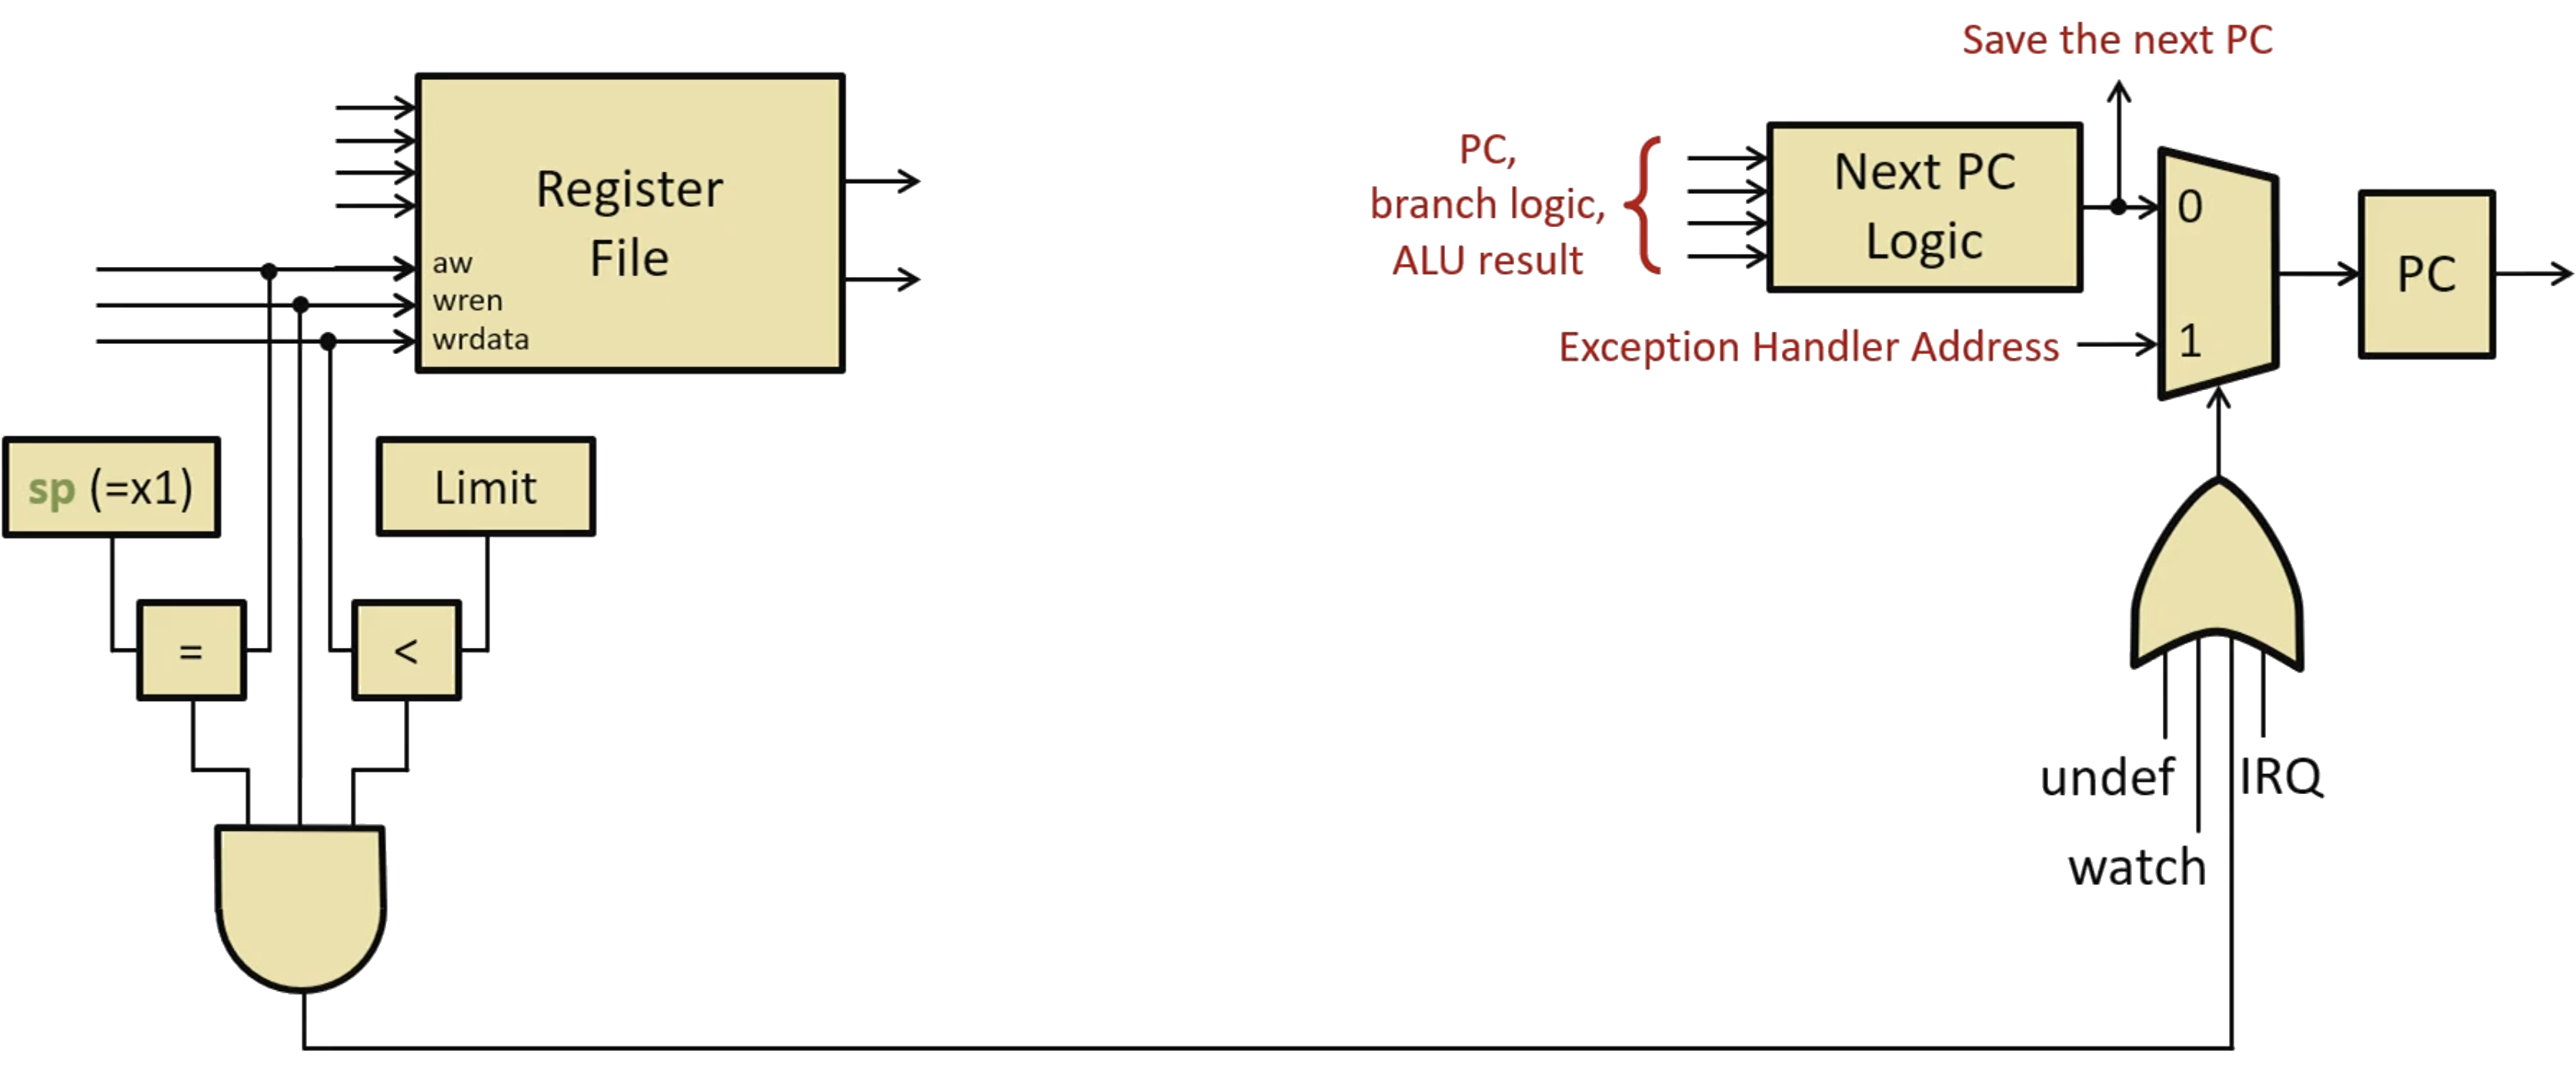
\includegraphics[width=0.75\textwidth]{chapters/chapter2d/images/stack_full.png}
\end{center}
\subsection{Writing Handlers is Very Very Tricky}
To write the exception handler for the stack-full detection, we \textbf{cannot} use the stack. \\
Writing interrupt or exception handlers is inherently complex, particularly due to the restriction that the stack cannot be used. Additionally, many registers may be untouchable during execution. This necessitates careful design to handle these constraints. 

\subsubsection*{Challenges}
\begin{itemize}
    \item[-] \textbf{Stack usage}: Direct stack usage is prohibited, necessitating alternative storage mechanisms.
    \item[-] \textbf{Register constraints}: In many cases, touching any general-purpose register is disallowed.
\end{itemize}

\subsubsection*{Solutions}
Various architectures provide mechanisms to address these challenges:
\begin{itemize}
    \item[-] \textbf{Reserved Registers}: As seen in MIPS, specific registers such as \texttt{\$k0} and \texttt{\$k1} are reserved for handler use.
    \item[-] \textbf{Shadow Registers}: Early processors (e.g., x86 and earlier) employ shadow registers for temporary data storage.
    \item[-] \textbf{Safe Stack Switching}: Architectures like x86 allow automatic switching to a predefined safe stack.
\end{itemize}

\subsubsection*{RISC-V Solution}
The RISC-V architecture employs a dedicated Control and Status Register (CSR) called \texttt{mscratch} (Machine Scratch) to facilitate temporary data storage during handler execution. The \texttt{mscratch} register can:
\begin{itemize}
    \item[-] Store one word of data for temporary usage.
    \item[-] Hold a pointer to an empty memory region or a predefined safe stack.
\end{itemize}

\subsection{Speaking of the Stack...}
\textit{Speaking of the stack, when writing assembly code, we often ask ourselves: is the code on the right side as valid as the code on the left side? The answer is yes, but handling stack overflow, as we were planning to do using a watchpoint, would've made it impossible to write the right version.} \\
\begin{minipage}[htp]{0.45\textwidth}
\begin{assembly}
funct:
    addi sp, sp, -12
    sw   ra, 0(sp)
    sw   s0, 4(sp)
    sw   s1, 8(sp)
    ... etc. ...
    lw   ra, 0(sp)
    lw   s0, 4(sp)
    lw   s1, 8(sp)
    addi sp, sp, 12
    ret
\end{assembly}    
\end{minipage}
\hfill
\vline
\hfill
\begin{minipage}[htp]{0.45\textwidth}
\begin{assembly}
funct:
    sw   ra, -12(sp)
    sw   s0, -8(sp)
    sw   s1, -4(sp)
    addi sp, sp, -12
    ... etc. ...
    addi sp, sp, 12
    lw   ra, -12(sp)
    lw   s0, -8(sp)
    lw   s1, -4(sp)
    ret
\end{assembly}
\end{minipage}

\section{Protection: I/Os Are Not for Everyone}
The system enforces restricted access to I/O peripherals to ensure security and proper operation. 
\begin{center}
    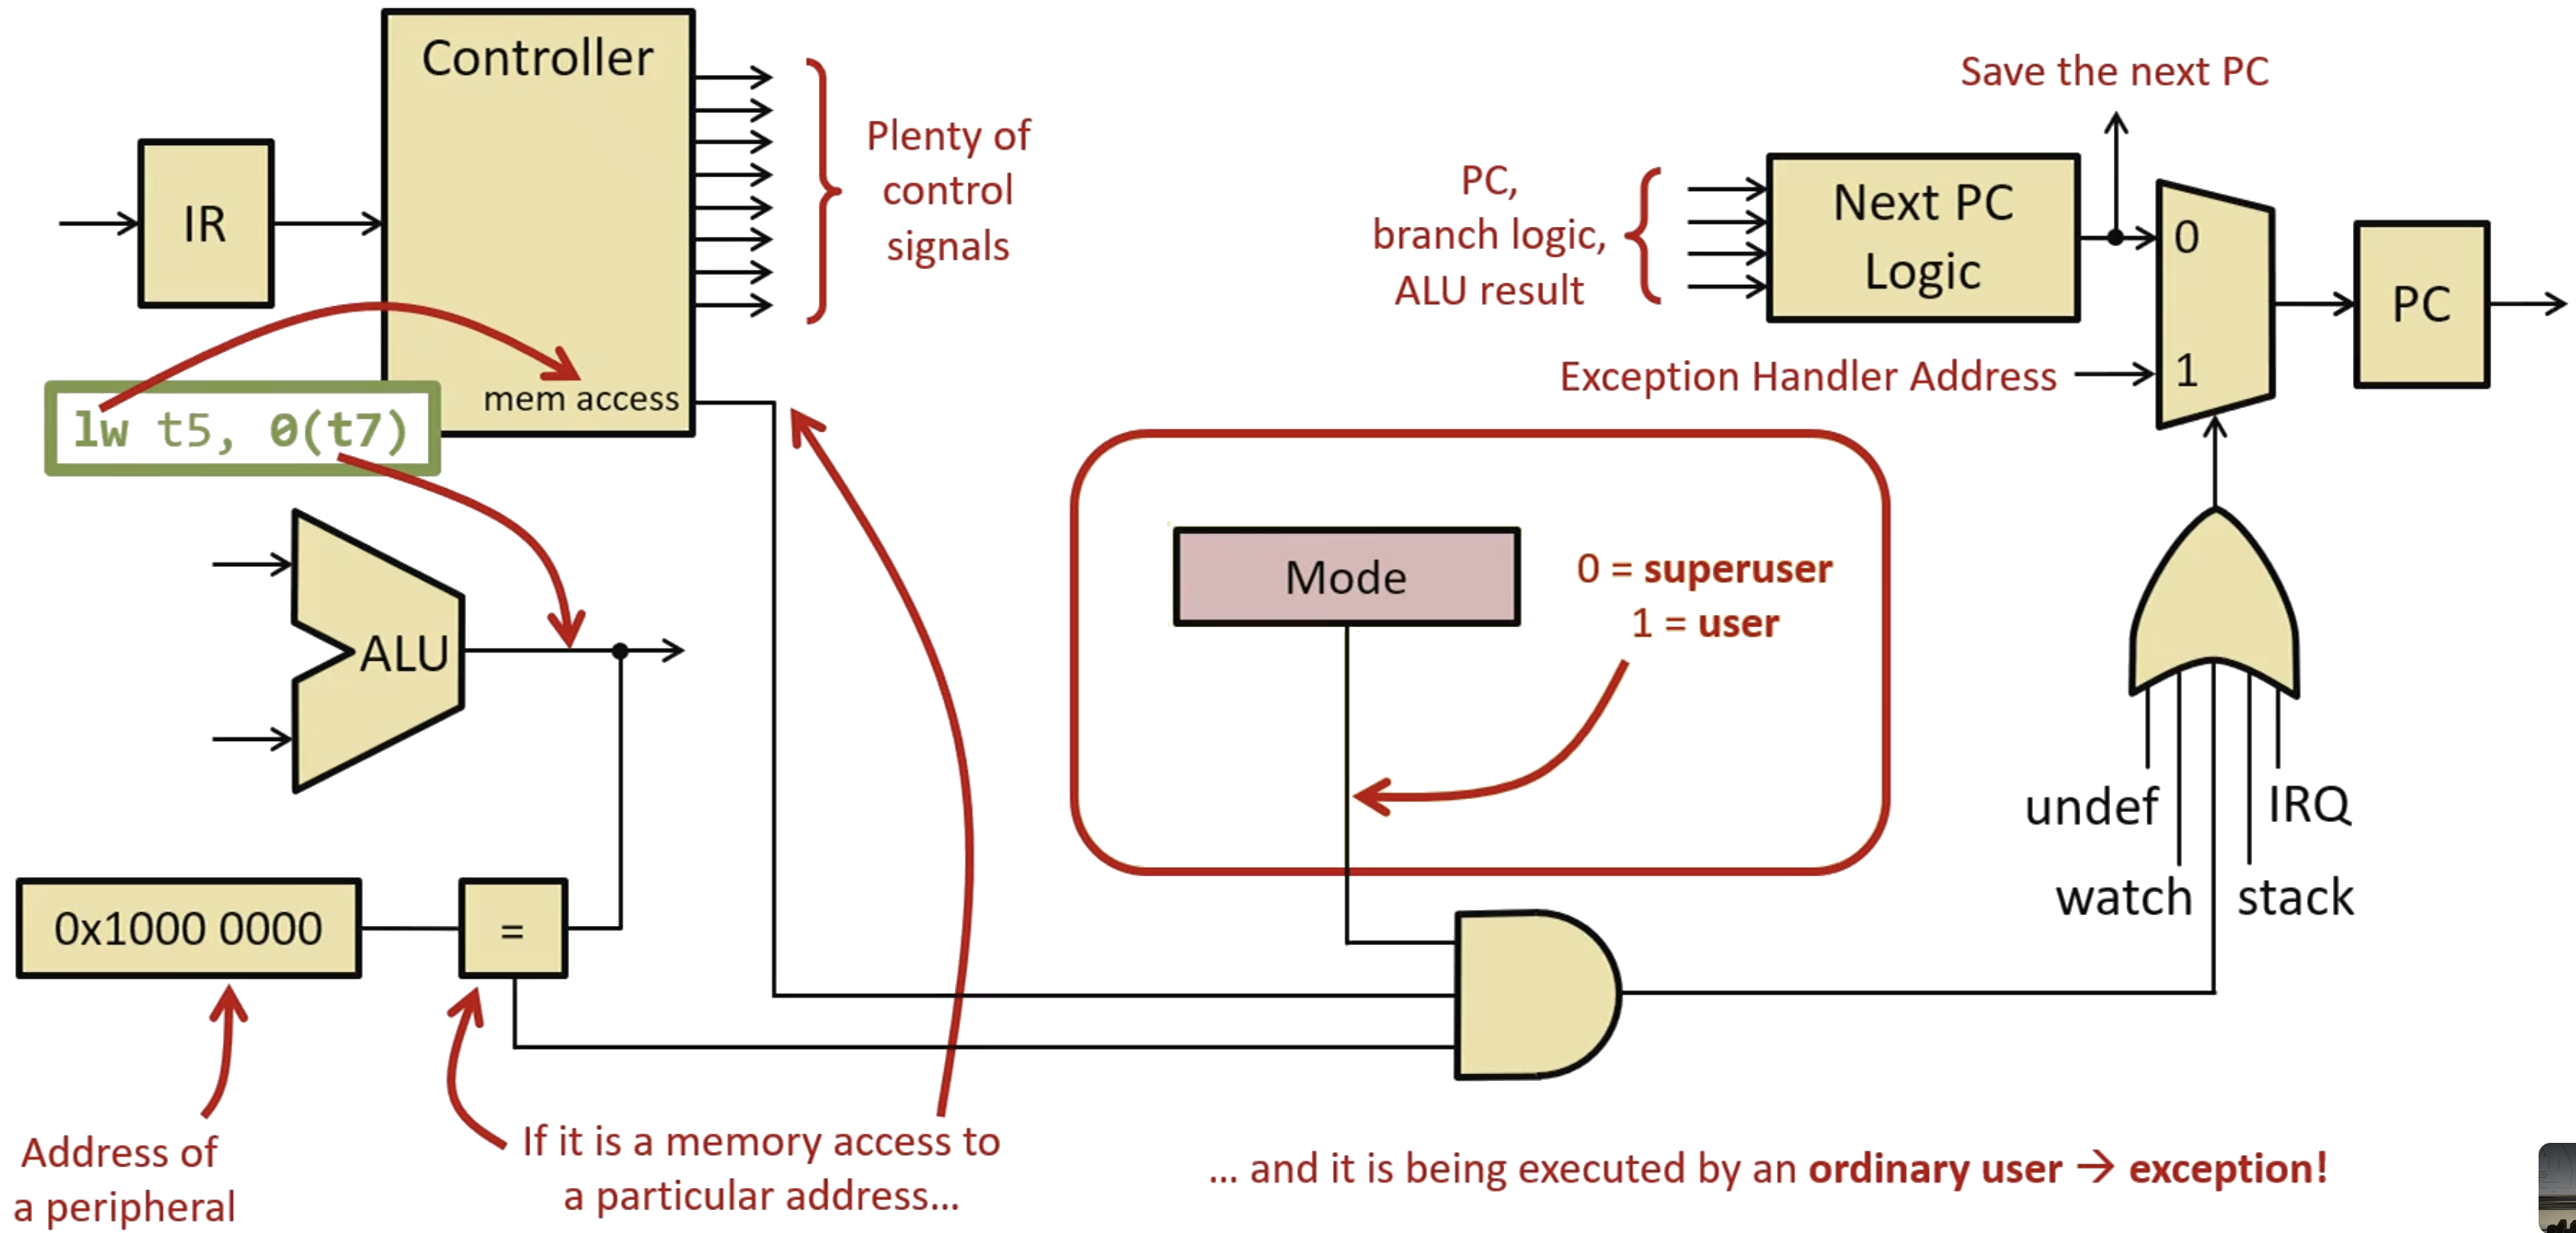
\includegraphics[width=0.65\textwidth]{chapters/chapter2d/images/admin.png}
\end{center}
\begin{itemize}
    \item[-] \textbf{Instruction Register (IR):} Holds the current instruction, e.g., \texttt{lw t5, 0(t7)}, which specifies a memory access operation.
    \item[-] \textbf{Controller:} Generates the necessary control signals to manage instruction execution and memory access.
    \item[-] \textbf{ALU (Arithmetic Logic Unit):} Computes addresses and performs arithmetic or logical operations. In this case, it calculates the effective memory address for the load instruction.
    \item[-] \textbf{Peripheral Address Check:} Compares the computed address against a predefined address (\texttt{0x10000000}) to determine if the operation targets a restricted peripheral.
    \item[-] \textbf{Privilege Mode:} Maintains the execution mode:
        \begin{itemize}
            \item \texttt{0:} Superuser mode.
            \item \texttt{1:} User mode.
        \end{itemize}
        If a user-mode instruction attempts to access a restricted address, an exception is triggered.
    \item[-] \textbf{Exception Handling:} Routes control to an exception handler when a violation occurs. This involves:
        \begin{itemize}
            \item Saving the next program counter (PC).
            \item Redirecting execution to the exception handler address.
        \end{itemize}
    \item[-] \textbf{Interrupt Sources:} Includes various triggers such as undefined instructions (\texttt{undef}), IRQ, watchpoints, and stack violations, which can cause exceptions.
\end{itemize}

\noindent This mechanism ensures secure memory access, prevents unauthorized peripheral usage, and enforces privilege separation to maintain system security.

\subsection{Levels of Privilege: Processor Modes}
Modern processors are designed with multiple levels of privilege to ensure proper execution of user programs and operating system tasks. These levels are referred to as \textbf{processor modes} and include:
\vspace{5px}
- \textbf{Distinction Between Processor Modes:} \\
\begin{itemize}
    \item \textbf{User Mode:} For executing user programs.
    \item \textbf{Kernel/Supervisor/Executive Mode:} For handling operating system tasks and privileged instructions.
    \item \textbf{RISC-V:} Includes up to three modes: Machine, Supervisor, and User.
\end{itemize}
\vspace{5px}
- \textbf{Processor State and Privilege Levels:} \\ 
\begin{itemize}
    \item Some parts of the processor state are \textit{readable by all} privilege levels, but can only be \textit{written to} by the highest privilege levels.
    \item Examples include:
    \begin{itemize}
        \item The \textbf{current mode register}.
        \item Configuration registers (e.g., memory hierarchy configuration).
    \end{itemize}
\end{itemize}
\vspace{5px}
- \textbf{Methods for Switching Between Modes:} \\ 
\begin{itemize}
    \item Processors provide:
    \begin{itemize}
        \item A \textit{dedicated instruction} to trigger a software exception.
        \item An instruction to reset the mode.
    \end{itemize}
    \item In RISC-V:
    \begin{itemize}
        \item \texttt{ecall} is used for system calls.
        \item \texttt{mret/sret} are used to return from exceptions.
    \end{itemize}
\end{itemize}

\subsection{Processor Tasks on Exception}
When an exception is raised, the processor typically performs a series of tasks. These tasks depend on the processor architecture and the type of exception. The main steps include:

\begin{enumerate}
    \item \textbf{Mask further interrupts:} Prevent additional interrupts to ensure the exception is handled correctly.
    \item \textbf{Save the Exception Program Counter (EPC):} Store the address of the instruction causing the exception.
    \item \textbf{Save exception details:} Record the reason or context for the exception.
    \item \textbf{Modify privilege level:} Switch to a higher privilege level as exception handlers often run in privileged mode.
    \item \textbf{Free up registers:} Temporarily save or copy certain registers to shadow registers if supported.
    \item \textbf{Jump to the exception handler:} Transfer control to the handler routine.
\end{enumerate}

\noindent After the exception is handled, most or all of these tasks are \textit{implicitly reverted} using special instructions. For example, the \texttt{mret} instruction in RISC-V resets the privilege level and re-enables interrupts. \\
\vspace{5px}
Some tasks, however, must be \textit{explicitly reverted} by the handler. For instance, programmers may need to unmask further interrupts manually as soon as it is safe to do so.

\subsection{Priorities in Interrupt Handling}

\textit{Interrupt controllers} play a critical role in managing priorities, determining which interrupt is more urgent to serve. \\

While hardware mechanisms primarily affect the order in which Interrupt Requests (IRQs) are presented to the processor, there are scenarios where it is desirable to serve a high-priority interrupt even while handling a lower-priority one.

However, there is a limitation: the processor architecture typically provides only a single \texttt{mepc} (Machine Exception Program Counter) and \texttt{mcause} (Machine Cause Register) register. Consequently, as soon as the processor accepts an interrupt, it must disable further interrupts to preserve critical state information.
\subsubsection*{Potential Solutions}
To address this limitation, we can implement the following strategies:
\begin{itemize}
    \item \textbf{Saving State:} Critical information about the interrupt (\texttt{mepc}, \texttt{mcause}, \texttt{mstatus}) can be saved on a safe stack. This ensures that Control and Status Registers (CSRs) can be overwritten by subsequent interrupts without losing essential context.
    \item \textbf{Re-enabling Interrupts:} The \texttt{mstatus} register can be manually updated to re-enable interrupts without returning from the handler, allowing higher-priority interrupts to preempt the current one.
\end{itemize}

\subsection{More challenges in Writing Exception Handlers}

Writing exception handlers is a complex and challenging task due to the following reasons:

\begin{itemize}
    \item \textbf{Stack Constraints:} In some cases, the stack cannot be used, such as when the exception arises from a stack overflow.
    \item \textbf{Non-Interruptibility:} Exception handlers may not be interruptible if they rely on static locations to save data, including registers like \texttt{mscratch}, making them non-reentrant.
    \item \textbf{System Limitations:} The system might be unable to tolerate prolonged interruptions, for instance, when I/O buffers risk filling up due to unserved interrupts.
\end{itemize}

Additionally, buggy \textbf{device drivers} from peripheral vendors often run in privileged mode, invoked by the operating system's interrupt handler, and can destabilize the system. 

\section{Example - Back to Our A/D Converter}
Let's revisit the example of an A/D converter, which converts analog signals to digital data. This device is connected to the processor via an I/O port, and the processor reads the converted data from the device. \\
\begin{center}
    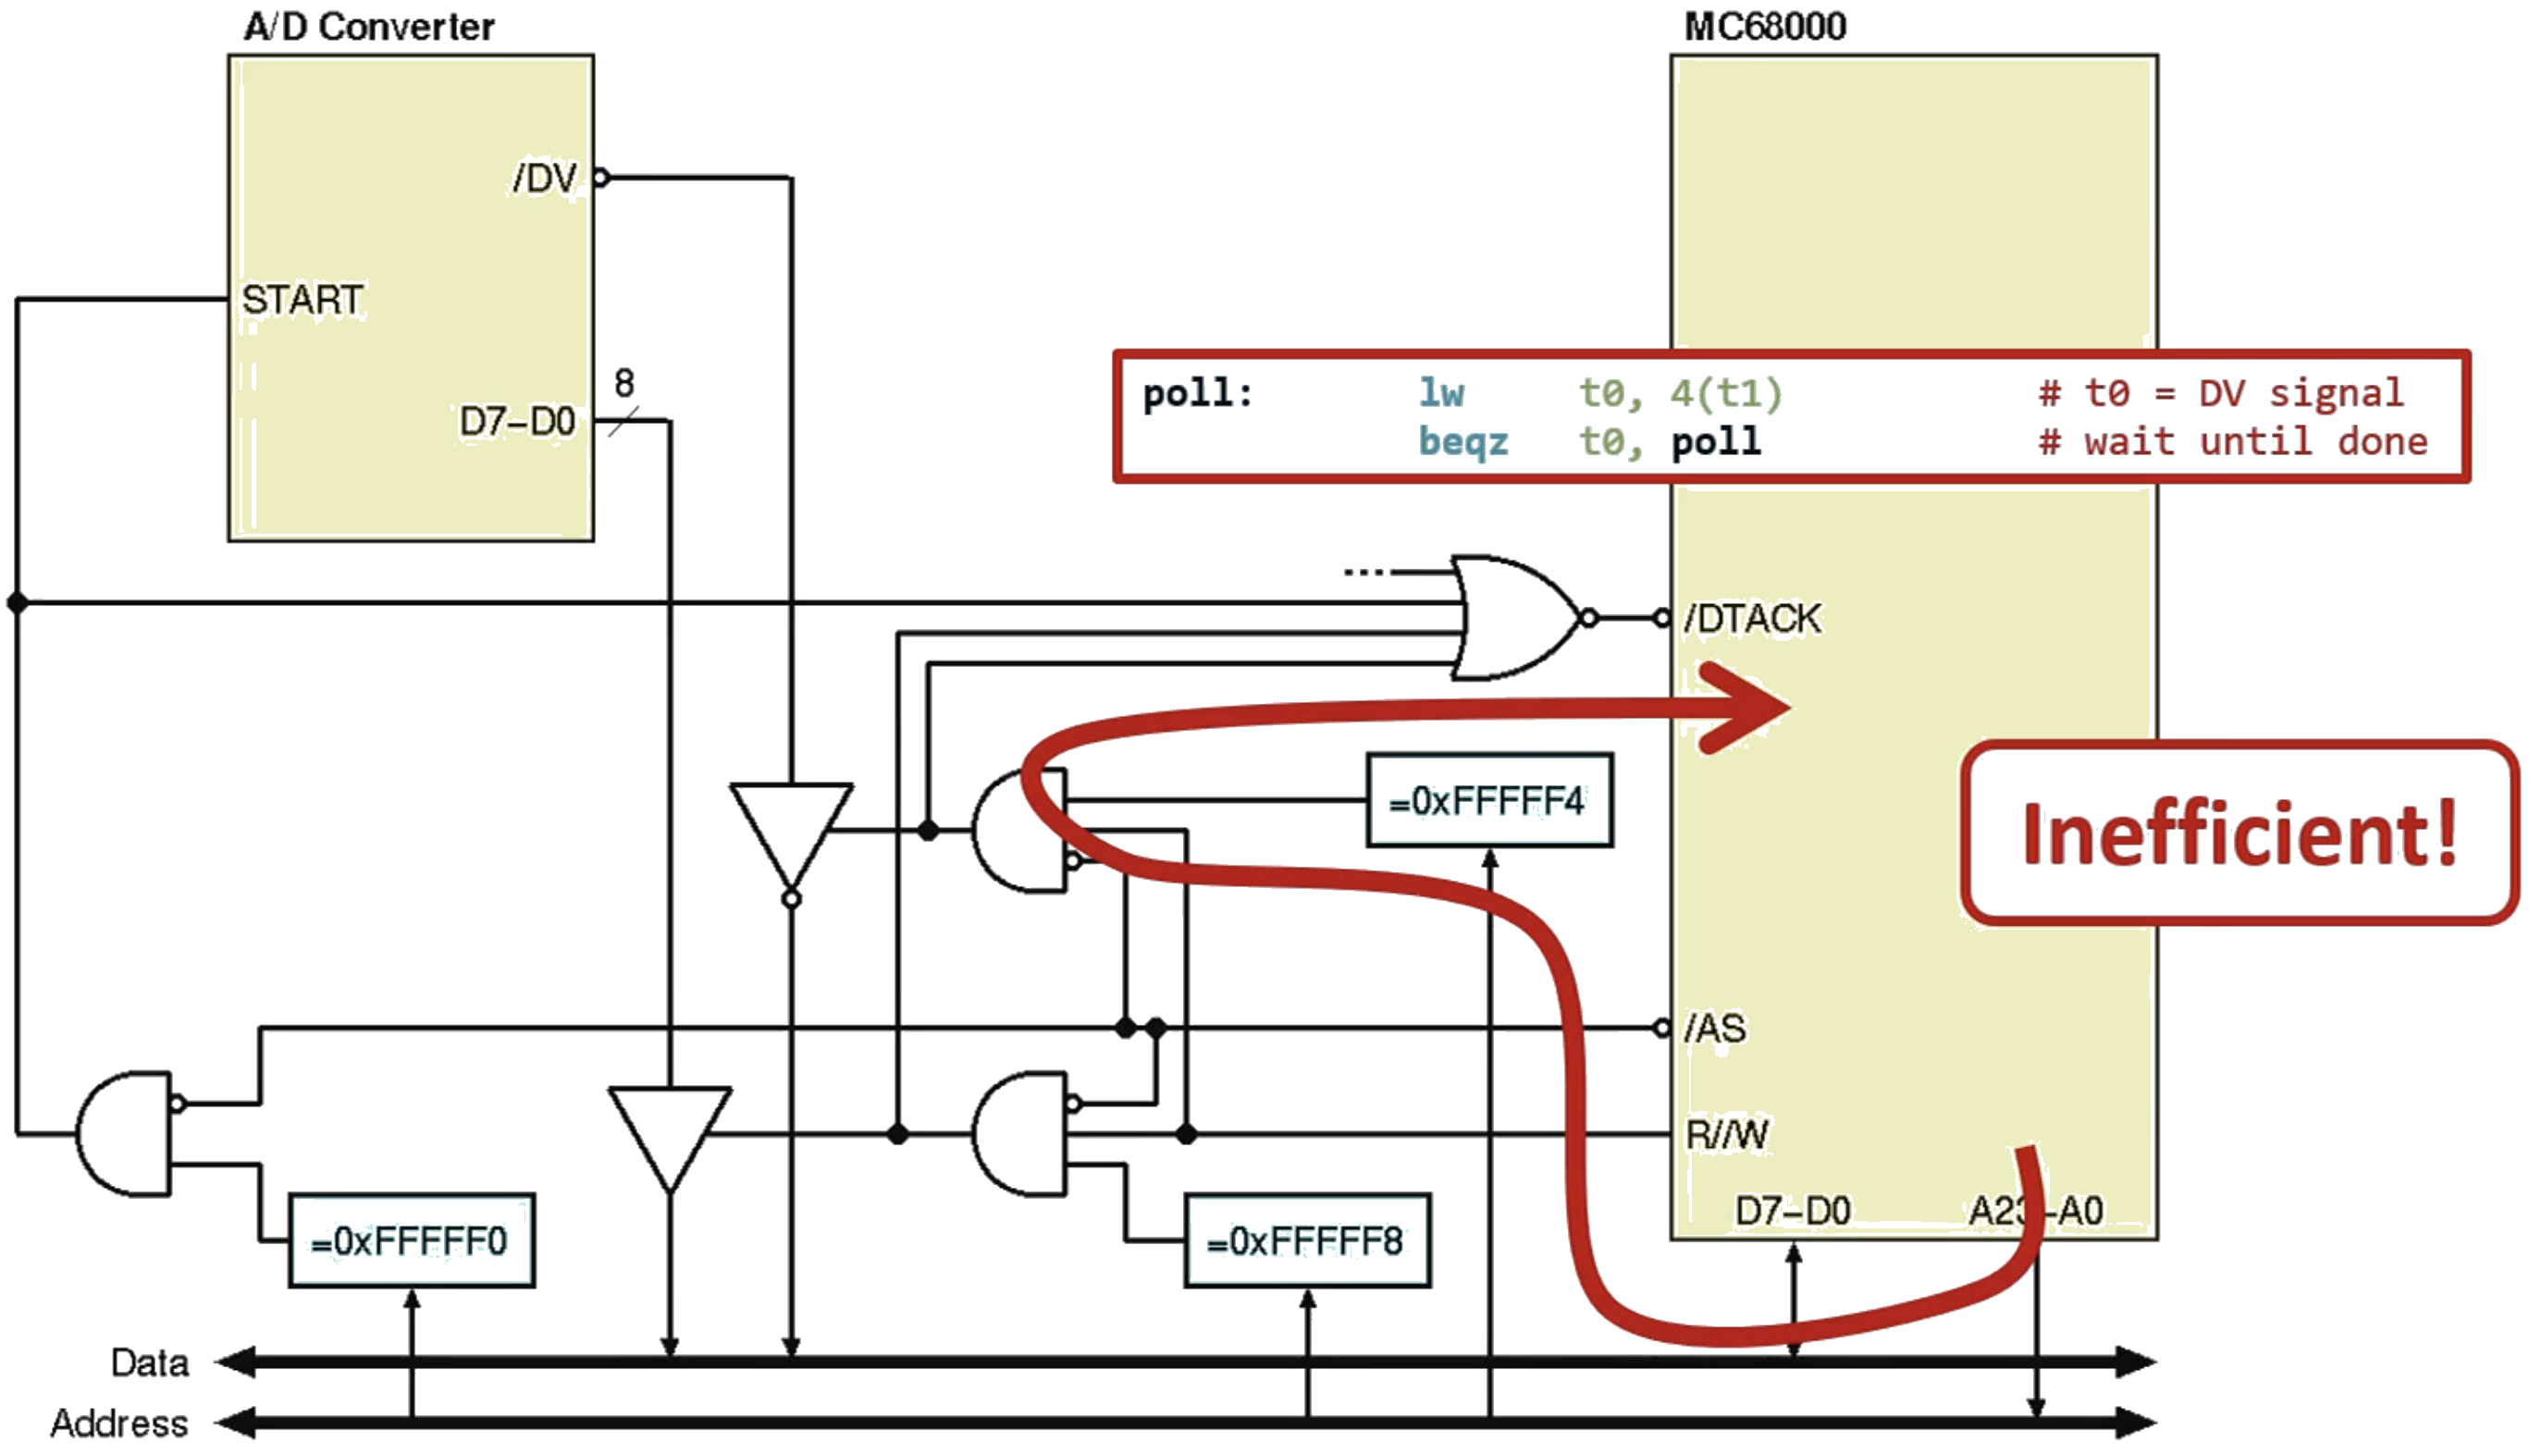
\includegraphics[width=0.65\textwidth]{chapters/chapter2d/images/adc.png}
\end{center}
\textit{Here though, we used to have an efficient approach to read the data from the A/D converter which was that we used to keep reading the Data Valid signal waiting for it to become active. (highly inneficient)} \\

\subsection{Simple IREQ and IACK Mechanism}

In an 8-bit processor with an internal interrupt controller, various \texttt{IREQ/IACK} signal pairs are used for I/O interrupt requests. For the Analog-to-Digital Converter (ADC), the following signals are assigned:

\begin{itemize}
    \item \textbf{\texttt{IREQ3}}: An input signal dedicated to the peripheral to request attention from the processor.
    \item \textbf{\texttt{IACK3}}: An output signal used by the processor to acknowledge the request and signal that it is being served.
\end{itemize}

The interaction between the peripheral and the processor can be described as follows:
\begin{center}
    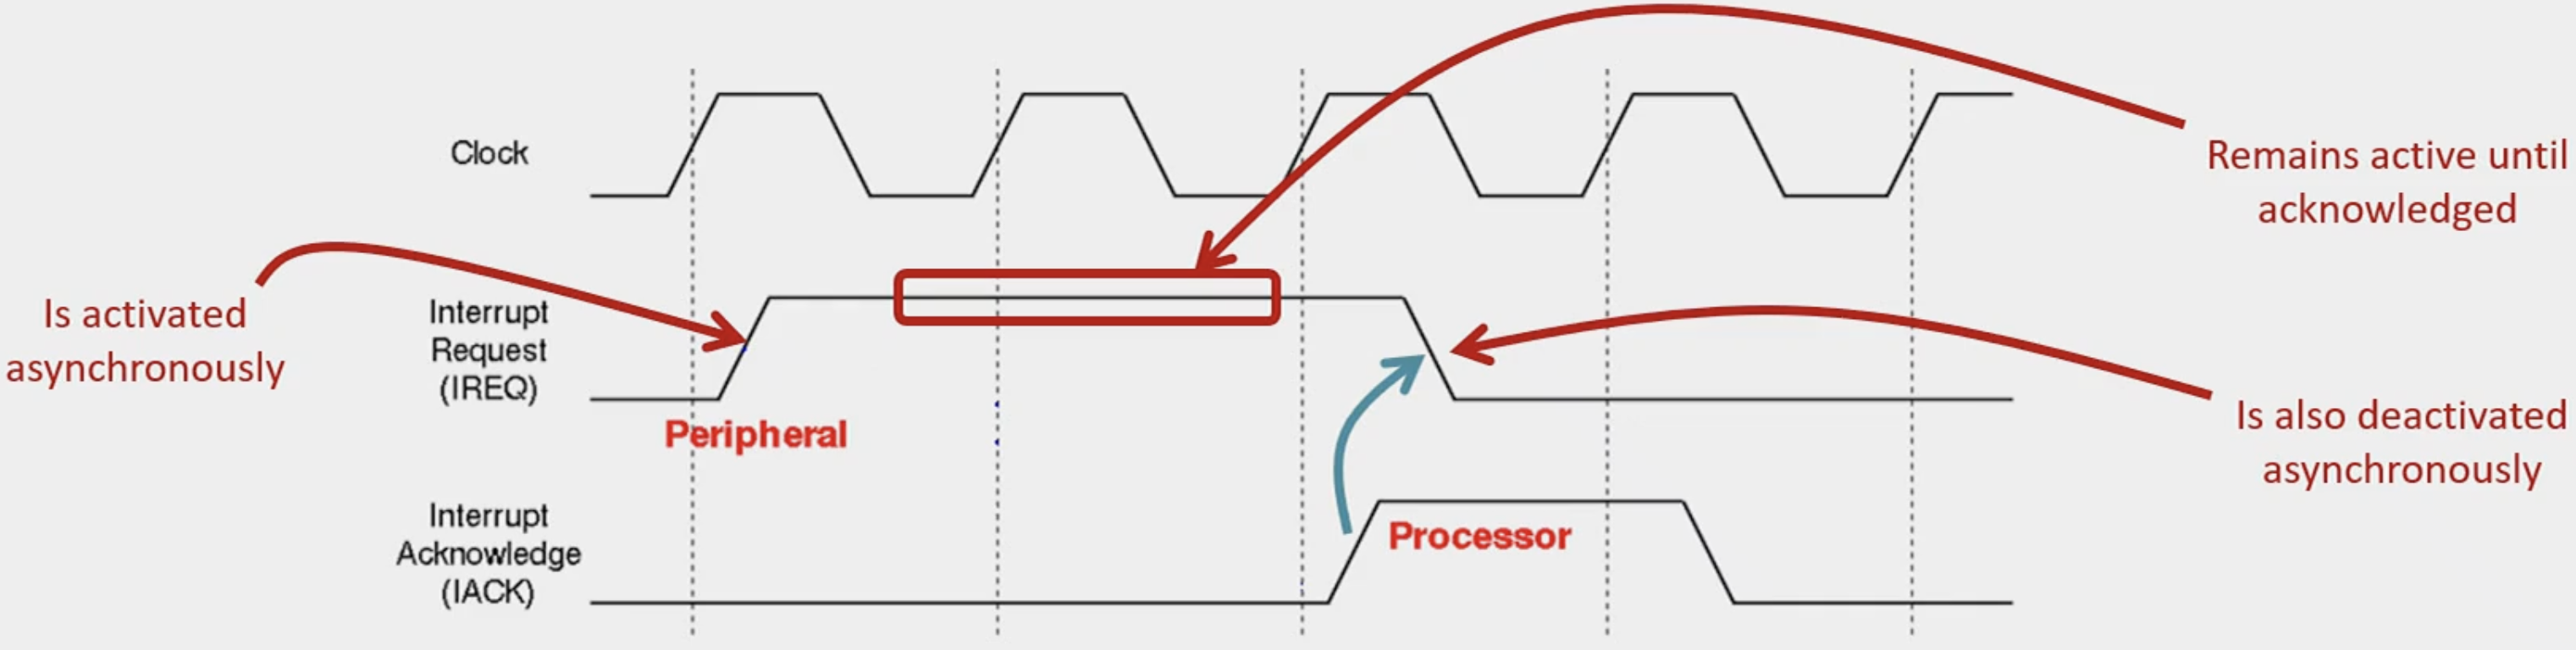
\includegraphics[width=0.75\textwidth]{chapters/chapter2d/images/mecanism.png}
\end{center}
\begin{enumerate}
    \item The interrupt request (\texttt{IREQ}) is activated asynchronously by the peripheral.
    \item The request remains active until it is acknowledged by the processor.
    \item Once the processor acknowledges the request using \texttt{IACK}, the interrupt is served, and \texttt{IREQ} is deactivated asynchronously.
\end{enumerate}

This mechanism ensures smooth communication and handling of interrupt-driven tasks between the peripheral and the processor.

\subsection{A/D Converter - startADC}
The \texttt{startADC} function initiates the Analog-to-Digital Conversion process by setting the \texttt{start} bit in the control register of the A/D converter. \\
\begin{assembly}
    lui t0, 0xfff
    addi t0, t0, 0xff0 #t0 = 0xfffff0
    sw zero, 0(t0)     # start conversion
    ret
\end{assembly}
\subsection{A/D Converter - Software:handler}
\begin{assembly}
handler:
    addi sp, sp, -120          # Save all registers but zero and sp
    sw x1, 0(sp)
    sw x3, 4(sp)
    ...                        # etc.
    sw x31, 116(sp)

    csrr s0, mcause            # Read exception cause
    bgez s0, handleExceptions  # Branch if not an interrupt (MSB = 0, 
                                # looks like zero or a positive number...)
    slli s0, s0, 1             # Get rid of the MSB of s0,
    srli s0, s0, 1             # so that what is left is the cause
    li s1, 11                  # s1 = external interrupt cause
    bne s1, s2, handleOtherInts # Branch if not an external interrupt

    jal readADC                # Returns a0 = ADC result
    jal insertIntoBuffer       # Gets a0 = value to add to a circular buffer

restore:
    lw x1, 0(sp)               # Restore all registers but zero and sp
    lw x3, 4(sp)
    ...                        # etc.
    lw x31, 116(sp)
    addi sp, sp, 120

    mret                       # Return from interrupt
\end{assembly}

\subsection{A/D Converter - insertIntoBuffer}
\begin{assembly}
.section .data
    .equ bufferSize, 1024              # Define buffer size (must be a power of two)
    .equ bufferBytes, bufferSize * 4  # Compute the total size in bytes for the buffer
    bufferPointer:
        .word 0                       # Initialize the pointer to index 0
    buffer:
        .space bufferBytes            # Allocate space for bufferSize * wordSize bytes

.section .text
insertIntoBuffer:
    la    t0, bufferPointer           # Load address of bufferPointer into t0
    lw    t1, 0(t0)                   # Load current buffer pointer into t1
    la    t2, buffer                  # Load base address of the buffer into t2
    slli  t3, t1, 2                   # Multiply buffer pointer (t1) by 4 to get byte offset
    add   t4, t2, t3                  # Add offset to buffer base address (= next word)
    sw    a0, 0(t4)                   # Store a0 into buffer at calculated position
    addi  t1, t1, 1                   # Increment buffer pointer by 1
    li    t5, bufferSize - 1          # Load bufferSize - 1 into t5 (mask for power of 2)
    and   t1, t1, t5                  # Apply bitwise AND to wrap around
    sw    t1, 0(t0)                   # Store updated buffer pointer
    ret                               # Return from the function
\end{assembly}
    \newpage
\subsection{A/D Converter - readADC}
\begin{assembly}
readADC: 
    li t0, 0xfffff0 # t0 = 0xfffff0
    lw a0, 8(t0) # get ADC data output
    ret
\end{assembly}
